\documentclass{article}

\usepackage{graphicx} % Required for inserting images
\usepackage[left=1in,right=1in,top=1in,bottom=1in]{geometry}
\usepackage{amsmath}
\usepackage{amsthm} %proof environment
\usepackage{amssymb}
\usepackage{amsfonts}
\usepackage{enumitem} %nice lists
\usepackage{verbatim} %useful for something 
\usepackage{xcolor}
\usepackage{setspace}
\usepackage{titlesec}
\usepackage{blindtext} % I have no idea what this is 
\usepackage{caption}  % need this for unnumbered captions/figures
\usepackage{natbib}
\usepackage{tikz}
\usepackage{hyperref}

\titleformat{\section}
{\bfseries\Large}
{Lecture \thesection:}
{5pt}{}

\begin{document}

\title{AM 275 - Magnetohydrodynamics: Lecture Notes}
\author{Dante Buhl}
\doublespacing

\newcommand{\wrms}{w_{\text{rms}}}
\newcommand{\bs}[1]{\boldsymbol{#1}}
\newcommand{\tb}[1]{\textbf{#1}}
\newcommand{\bmp}[1]{\begin{minipage}{#1\textwidth}}
\newcommand{\emp}{\end{minipage}}
\newcommand{\R}{\mathbb{R}}
\newcommand{\C}{\mathbb{C}}
\newcommand{\N}{\mathcal{N}}
\newcommand{\K}{\bs{\mathrm{K}}}
\newcommand{\m}{\bs{\mu}_*}
\newcommand{\s}{\bs{\Sigma}_*}
\newcommand{\dt}{\Delta t}
\newcommand{\dx}{\Delta x}
\newcommand{\tr}[1]{\text{Tr}(#1)}
\newcommand{\Tr}[1]{\text{Tr}(#1)}
\newcommand{\Div}{\nabla \cdot}
\renewcommand{\div}{\nabla \cdot}
\newcommand{\Curl}{\nabla \times}
\newcommand{\Grad}{\nabla}
\newcommand{\grad}{\nabla}
\newcommand{\grads}{\nabla_s}
\newcommand{\gradf}{\nabla_f}
\newcommand{\xs}{x_s}
\newcommand{\xf}{x_f}
\newcommand{\x}{\bs{x}}
\newcommand{\ts}{t_s}
\newcommand{\tf}{t_f}
\newcommand{\pt}{\partial t}
\newcommand{\pz}{\partial z}
\newcommand{\uvec}{\bs{u}}
\newcommand{\nvec}{\hat{\bs{n}}}
\newcommand{\jvec}{\bs{j}}
\newcommand{\bvec}{\bs{B}}
\newcommand{\B}{\bs{B}}
\newcommand{\evec}{\bs{E}}
\newcommand{\E}{\bs{E}}
\newcommand{\vort}{\bs{\omega}}
\newcommand{\F}{\bs{F}}
\newcommand{\T}{\tilde{T}}
\newcommand{\ez}{\bs{e}_z}
\newcommand{\ex}{\bs{e}_x}
\newcommand{\ey}{\bs{e}_y}
\newcommand{\thetahat}{\hat{\bs{\theta}}}
\newcommand{\rhat}{\hat{\bs{r}}}
\newcommand{\zhat}{\hat{\bs{z}}}
\newcommand{\eo}{\bs{e}_{\bs{\Omega}}}
\newcommand{\ppt}[1]{\frac{\partial #1}{\partial t}}
\newcommand{\pptwo}[2]{\frac{\partial^2 #1}{\partial #2^2}}
\newcommand{\ppthree}[2]{\frac{\partial^3 #1}{\partial #2^3}}
\newcommand{\pp}[2]{\frac{\partial #1}{\partial #2}}
\newcommand{\ddt}[1]{\frac{d #1}{d t}}
\newcommand{\DDt}[1]{\frac{D #1}{D t}}
\newcommand{\DD}[2]{\frac{D #1}{D #2}}
\newcommand{\ppts}[1]{\frac{\partial #1}{\partial t_s}}
\newcommand{\pptf}[1]{\frac{\partial #1}{\partial t_f}}
\newcommand{\ppz}[1]{\frac{\partial #1}{\partial z}}
\newcommand{\ddz}[1]{\frac{d #1}{d z}}
\newcommand{\dd}[2]{\frac{d #1}{d #2}}
\newcommand{\ppzetas}[1]{\frac{\partial^2 #1}{\partial \zeta^2}}
\newcommand{\ppzs}[1]{\frac{\partial #1}{\partial z_s}}
\newcommand{\ppzf}[1]{\frac{\partial #1}{\partial z_f}}
\newcommand{\ppx}[1]{\frac{\partial #1}{\partial x}}
\newcommand{\ppxi}[1]{\frac{\partial #1}{\partial x_i}}
\newcommand{\ppxj}[1]{\frac{\partial #1}{\partial x_j}}
\newcommand{\ppy}[1]{\frac{\partial #1}{\partial y}}
\newcommand{\ppzeta}[1]{\frac{\partial #1}{\partial \zeta}}


\maketitle 

\tableofcontents

\setlength{\parindent}{0pt}
\setcounter{section}{1}

\section{Hydrodynamics Review}

What is a fluid?
\begin{itemize}
    \item Its flows! 
    \item it deforms continuously
\end{itemize}

Categorization of fluids:
\begin{itemize}
    \item Compressible v. incompressible
    \item viscous v. inviscid
    \item + many more
\end{itemize}

\vspace{20pt}

\bmp{.49}
    \centering
    {\Large \textbf{Eularian}}
    \vspace{5pt}

    Rate of change at a given point, no bother for where the fluid goes. 
    \begin{gather*}
        \frac{\partial}{\partial t}\left(\cdot\right) 
    \end{gather*}
\emp
\hspace{5pt}
\bmp{.49}
    \centering
    {\Large \textbf{Lagrangian}}
    \vspace{5pt}

    Follows the particle, introduces the advection term
    \begin{gather*}
        \uvec\cdot\grad \left(\cdot\right)
    \end{gather*}
\emp

\vspace{20pt}
{\Large \textbf{Mass Conservation}}
\vspace{5pt}


In order to conserve mass we consider an arbitrary eularian volume (i.e. the
volume doesn't move with the flow). We then find the total mass which is equal
to the integral of the density over the volume, and then consider the flux of
mass through the boundary (change in mass over time). Using the divergence
theorem, we then have a conservation equation for mass. 

\begin{gather*}
    \ppt{}\int_D\rho dV = \int_{\partial D} \rho\uvec \cdot \eta dA\\
    \ppt{\rho} + \grad\cdot \rho\uvec = 0 \\
    \ppt{\rho} + \uvec\cdot\grad\rho + \rho\grad\cdot\uvec = 0\\
    \frac{D\rho}{Dt} = - \rho \grad\cdot\uvec
\end{gather*}

More importantly, if we consider an incompressible fluid, i.e. $\rho = \rho_0$,
we have very specifically,
\begin{gather}
    \grad \cdot \uvec = 0
\end{gather}


\vspace{20pt}
{\Large \textbf{Stresses}}
\vspace{5pt}

Stresses can be divided into two catagories, body forces and surface forces.
Body forces are forces such as gravity and the electric force, which surface forces are
forces such as normal force and friction. 

\vspace{20pt}
{\Large \textbf{Newtons Second Law}}
\vspace{5pt}
Newton's second law 
\begin{gather*}
    \ppt{p} = \sum_i F_i
\end{gather*}
where $p$ here is the momentum of a fluid parcel. In actuality, the momentum can
be written as $p = \int_D \rho\uvec dV$. So, 
\begin{gather*}
    \DDt{}\int_D \rho\uvec dV = \int_D \rho \bs{g} dV + (\text{other body
    forces}) + \grad \cdot \bs{\tau}\\
    \rho\DDt{\uvec} = \rho F + \grad\cdot\bs{\tau}
\end{gather*}
where $\bs{\tau}$ is the stress tensor acting on the fluid parcel. Surface
forces are then introduced into this stress tensor. First and foremost, surface
pressure is introduced along the stress tensor. 
\begin{gather*}
    \tau_{ij} = -p\delta_{ij} + \sigma_{ij}
\end{gather*}
where $\sigma_{ij}$ is the deviatoric stress tensor and is responsible for the
off-diagonal components of the stress tensor. Some components are the velocity
gradient tensors, $\ppxj{u_i}$ and $\ppxi{u_j}$. Each of these has a symmetric
compoenent and an antisymmetric componenet. 
\begin{gather*}
    \ppxj{u_i} = \frac{1}{2}\left(\ppxj{u_i} + \ppxi{u_j}\right) +
    \frac{1}{2}\left(\ppxj{u_i} - \ppxi{u_j}\right)
\end{gather*}
The first term is labeled symmetric and denoted $e_{ij}$ while the second
component is the rotation componenet. 



\section{Continuing Review of the Kinematic Equations}

\subsection{Obtaining the Navier-Stokes equation}

Decomposition of the deviatoric stress tensor reveals a 4th order tensor with 81
components.
\begin{gather*}
    \bs{\sigma}_{ij} = \bs{A}_{ijkl}\bs{e}_{kl}
\end{gather*}
In order to reduce the complexity of the system, we make some assumptions about
the tensor $\bs{A}_{ijkl}$. First, we state that this tensor must be isotropic,
i.e. that it doesn't care about the direction of the stress with respect to the
coordinate system it is in. We have, 
\begin{gather*}
    \bs{A}_{ijkl} = \mu \bs{\delta}_{ij}\bs{\delta}_{kl} +
    \mu'\bs{\delta}_{ik}\bs{\delta}_{jl} +
    \mu''\bs{\delta}_{il}\bs{\delta}_{jk}
\end{gather*}
Next, we assume that this tensor must be symmetric. This reduces the complexity
down to two coefficients, $\mu$, the viscosity, and $\mu'$ which is the bulk viscosity. 

In order to obtain the Navier-Stokes equation, we require the Stokes assumption
which postulates that the diagonal components of the deviatoric stress tensor
are zero, i.e. $\bs{\sigma}_{ii} = 0$. 
\begin{gather*}
    \bs{\sigma}_{ij} = 2\mu\left(\bs{e}_{ij} -
    \frac{1}{3}\left(\grad\cdot\uvec\right)\bs{\delta}_{ij}\right)    \\
    \bs{\tau}_{ij} = -p\bs{\delta}_{ij} + 2\mu\left(\bs{e}_{ij} -
    \frac{1}{3}\left(\grad \cdot \uvec\right)\bs{\delta}_{ij}\right)
\end{gather*}
Therefore, when we take the divergence of this stress tensor we obtain the
Navier-Stokes equation:
\begin{gather*}
    \rho\DDt{\uvec} = \rho\bs{F} - \grad p + \mu\left[ \grad^2 \uvec +
    \frac{1}{3}\grad \left(\grad \cdot \uvec\right)\right]
\end{gather*}
Of course, when working in an incompressible framework (i.e. $\grad\cdot\uvec =
0$), we have that part of the diffusive term disappears from the equation,
resulting in the commonly used equation:
\begin{gather}
    \label{eq:NS}
    \DDt{\uvec} = \bs{F} - \frac{1}{\rho_0}\grad p + \nu\grad^2 \uvec
\end{gather}
Additional terms are included in this equation as necessary to model relevant
physics of various fluid systems. For example, if in a rotating frame we include
the coriolis force $2\Omega(\bs{e}_{\Omega} \times \uvec)$, if some component of
the fluid is stratified we need some buoyancy forcing $T/N^2\bs{e}_z$. And most
relevant, there might be magnetic forces which affect the fluid, in which case
we obtain the MHD equations. 

\subsection{Vorticity equation}

Vorticity is a quantity related to the fluid field which can be very important
to the scientific study of fluid dynamics. The vorticity is obtained by taking
the curl of the velocity field. 
\begin{gather*}
    \bs{\omega} = \grad \times \uvec
\end{gather*}
The vorticity has an evolution-advection equation just as the velocity field
does, and in fact the vorticity equation is obtained by taking the curl of the
Navier-Stokes equations.

\begin{gather*}
    \grad\times\eqref{eq:NS}\\
    \DDt{\vort} =  \left(\vort\cdot\grad\right)\uvec +
    \vort\left(\grad\cdot\uvec\right) + \grad\times\F -
    \frac{1}{\rho^2}\grad\rho\times\grad p + 
    \nu\grad^2\vort 
\end{gather*}

If the flow is incompressible, one of the vortex stretching terms disappears.
Generally, the first two right hand terms are vortex stretching/tilting/speed-up
terms. Then the pressure and density gradient cross product is the baroclinicity
term, the curl of $\F$ is the forcing of vorticity, and finally, we have a
viscous diffusion of vorticity which behaves similarly to the diffusion of
velocity. 


Baroclinicity is perhaps the most unintuitive term in this equation, and it
simply represents the creation of rotation in the fluid when there is a
disalignment between the pressure and density gradients in the fluid. 

Some fluid dynamicists prefer to study the vorticity equation, especially for
rotating flows where voricites and cyclones are common phenomenon in the flow
field. 

\subsection{Rotation}

In the presence of rotation, the coriolis force becomes relevant as the motion
of a fluid particle is deflected due to the rotation of the cordinate frame.
That is, our equations are modified such that, 
\begin{gather*}
    \ppt{\bs{q}}_F = \ppt{\bs{q}}_R + 2\bs{\Omega}\times \bs{q} -
    \bs{\Omega}^2\bs{R}
\end{gather*}

This also introduces an additional term to the vorticity equation which looks
like, $+\left(2\bs{\Omega}\cdot\grad\right)\uvec$. 


\section{Conservation of Energy and Maxwell's equations}

\subsection{Conservation of Energy}

The equation of state chosen for a particular problem is a source of physics
which affects the solutions of a given PDE. The incompressible equation of
state is used very commonly as an equation of state. Another common one is the
ideal gas law $pV = \rho RT$. 

In order to understand the origin and importance of the equation of state, the
laws of thermodynamics are needed. 

The first law of thermodynamics states, 

\begin{gather*}
    \ppt{e} = \ppt{W} + \ppt{Q}
\end{gather*}
where $e$ is the internal energy, $W$ is work done on the system, and $Q$ is
heat flux into the system. However, for a fluid flow taken from a Lagrangian
perspective, we must modify this law of thermodynamics. It must include the
energy given by the velocity field. 

\begin{gather*}
    \DDt{}\int_D \rho\left(e+\frac{1}{2}\uvec^2\right)dV = \int_D \rho
    \F\cdot\uvec dV + \int_{\partial D} \bs{\tau}\cdot\uvec dS - \int_{\partial
    D} \bs{q}\cdot dS \\
    \rho\DDt{}\left(e+\frac{1}{2}\uvec^2\right) = \rho\F\cdot\uvec +
    \grad(\bs{\tau}\cdot\uvec) -
    \grad\cdot\bs{q} 
\end{gather*}

Next, we obtain a mechanical energy equation by dotting $\uvec$ by the
Navier-Stokes equation and adding $\uvec^2/2 \cdot \DDt{\rho}$
\begin{gather*}
    \DDt{\rho\uvec^2/2} = \rho\F\cdot\uvec -
    \uvec\cdot\left(\grad\cdot\bs{\tau}\right) + \ldots\\
    \uvec\cdot\left(\grad\cdot\bs{\tau}\right) = 
    \Phi = 2\mu\left[\bs{e}_{ij} -
    \frac{1}{3}(\grad\cdot\uvec)\bs{\delta}_{ij}\right]
\end{gather*}

Finally, we obtain an energy equation with a positive definite dissipation term
$\Phi$ which acts purely to remove energy from the system. 
\begin{gather*}
    \rho\DDt{e} = -\grad \cdot \bs{q} - p\left(\grad\cdot\uvec\right) + \Phi
\end{gather*}

The Second law of Thermodynamics also plays an important role in the
conservation of energy. The ssecond law makes statements about the entropy of a
system, $S$.
\begin{gather*}
    dS = \frac{dq}{T}\\
    TdS =  de + pdV\\
    T\ddt{S} = \ddt{e} - \frac{p}{\rho^2}\ddt{\rho}\\
    \rho \DDt{S} = - \frac{\grad \cdot \bs{q}}{T} + \frac{k}{T^2}|
    \grad T|^2 + \mu\frac{\Phi}{T}
\end{gather*}
Essentially, since both $|\grad T|^2$ and $\Phi$ are positive definite terms and
their coefficients are positive definite, it must be that the entropy of a
system can only increase ``on average'' (curse the statisticians). 

\subsection{Introducing Maxwell's Equations}

Electricity and Magnetism are very closely related to one another and governed
by a main set of governing equations. The main variables which we consider are a
position vector, $\bs{x}$, a velocity field, $\uvec$, density $\rho$, pressure
$p$, time $t$, temperature $T$, magnetic field (magnetic flux density) $\bvec$,
magnetic field strength $\bs{H}$, electric field $\bs{E}$, electric displacement
$\bs{D}$, electric current density $\bs{j}$, and charge density $\rho_e$. 

Alongside these variables, we have constants describing components of
electropmangetism: permitivity $\varepsilon$, permeability $\mu$, and
conductivity $\sigma$. Permitivity describes the charge requirement for a
specific electric field, i.e. large $\varepsilon$ implies a larger charge is
needed for a specific electric field. Permeability describes the current
requirement for a specific magnetic field, i.e. large $\mu$ implies a smaller
current is needed to obtain a specific magnetic field. 

Consitutive relationships describe the relationships between specific
electromagnetic quantities. 
\begin{gather*}
    \bs{H} = \frac{\bvec}{\mu}, \text{ for an isotropic permeability}\\
    \bs{D} = \varepsilon \bs{E}, \text{ for an isotropic permitivity}
\end{gather*}
where generally, we take $\mu = \mu_0$ and $\varepsilon = \varepsilon_0$ where
$q_0$ is taken from a vacuum. 

Now we write Maxwell's equations in their differential form:
\begin{align*}
    &\grad\cdot\bvec = 0, \text{ Gauss' law for magnetism}
    & \grad \cdot \bs{E} = \frac{\rho_e}{\varepsilon_0}, \text{ Gauss' law}\\
    &\grad \times \bs{E} = -\ppt{\bvec}, \text{ Faraday's law}
    &\grad \times \bvec = \mu_0\left(\bs{j} + \varepsilon_0\ppt{\bs{E}}\right),
    \text{ Ampere's Law of induction}
\end{align*}

They can be written in their integral form as well: 
\begin{align*}
    &\oint_{\partial D} \bvec\cdot\bs{dA} = 0 
    & \oint_{\partial D} \bs{E}\cdot\bs{dA} = \frac{q}{\varepsilon_0}\\
    &\oint_L \bs{E}\cdot\bs{dL} = -\ppt{\phi_{B}} 
    & \oint_L\bvec\cdot\bs{dL} = \mu_0\bs{j} + \mu_0\varepsilon_0\ppt{\phi_E}
\end{align*}
where $\phi_B = \int_S \bvec\cdot\bs{dA}$ is the total magnetic fluid, and 
$\phi_E = \int_S \bs{E}\cdot\bs{dA}$ is the total electric flux. 


We cover their derivations in a brief sense also. Consider a positive point
charge which creates an electric field. This imposes a force acting on any other
point charge in the field. This force is called Coulomb force given by $F =
q_1q_2/(4\pi\varepsilon r^2)$. Thus we have a given electric field of strength
$E/q = q_1/(4\pi\varepsilon r^2)$. We obtain the total electric flux $\phi_E$ 

\begin{gather*}
    d\phi_E = \bs{E}\cdot\bs{dA}\\
    \phi_E = \oint_S\frac{q_1}{4\pi\varepsilon r^2}\cdot\bs{dA}\\
    \phi_E = \frac{q_1}{4\pi\varepsilon r^2}\oint_S\bs{dA}\\
    \phi_E = \frac{q_e}{\varepsilon}
\end{gather*} 
where $q_e$ in the final equation is given by the sum of all point charges
enclosed in the closed volume, i.e. $q_e = \sum_i q_i$. Notice that $q_e$ can be
thought of as mass for point charges, i.e. the integral of the charge density
equals the total charge similar to how the integral of mass density equals the
total mass. It can be represented as a sum of point charges because point
cahrges are discrete and do not usually exist in a continuum. 

Finally, using the divergence theorem, 
\begin{gather*}
    \oint_S \bs{E}\cdot\bs{dA} = \int_V \grad\cdot\bs{E} dV\\
    q_e = \int_V \rho_{E} dV\\
    \grad\cdot\bs{E} = \frac{\rho_E}{\varepsilon}
\end{gather*}
Similarly, the same proof holds for Gauss' law of magnetism, only that monopoles
do not exist in magnetic fields, i.e. every source must have a sink. Therefore,
for an arbitraty volume it must be that the divergence of the magnetic field
must be zero: 
\begin{gather*}
    \div\bvec = 0
\end{gather*}

\section{Derivation of Maxwell's Equations: Continued}

\subsection{Faraday's Law of Induction}
    
The laws of electrodynamics are empiracle. Faraday realized that the EMF,
proportional to $\ppt{\bvec}$ and also the area of the coil. This led them to
deduce that EMF should be proportional to $\ppt{\phi_B}$. Note that EMF
represents the amount of work done per unit charge to move a charge from one
place to another, i.e. the electric potential difference. It has the units of
$Nm/C$ (Newton meters per Coulomb). 
\begin{align*}
    \text{EMF} = \oint_C\bs{E}\cdot\bs{dL} &= - \ppt{\phi_B} \\
    &= -\ppt{}\int_S\bvec\cdot\bs{dA}
\end{align*}
where here the RHS integral is not necessarily over a closed surface (because
the same integral over a closed surface must be zero). 

\subsection{Ampere's Law}

If there is a current moving through a wire, imagine a cross section going
through the wire (i.e. going through the page), there is a magnetic field around
the wire. The magnetic field can be described using the following integral form. 
\begin{gather*}
    \oint_L \bs{H}\cdot\bs{dL} = \bs{i}\\
    \oint_L\frac{\bvec}{\mu_0}\cdot\bs{dL} = \bs{i}\\
    \oint_L\bvec\cdot\bs{dL} = \mu_0\bs{i}\\
    \int_S\grad\times\bvec\cdot\bs{dA} = \mu_0\oint_A\bs{j}\cdot\bs{dA}\\
    \grad\times\bvec = \mu_0\bs{j}
\end{gather*}
Here is where Maxwell's contribution to Ampere's law is notable. Ampere assumed
that $\div{\bs{j}} = 0$, where Maxwell noticed that in some scenarios, this
is not necessarily true. Thus, he modified the equation to include displacement
currents. 

\begin{gather*}
    \ppt{\bs{D}} = \bs{j}_0\\
    \ppt{\varepsilon \bs{E}} = \bs{j}_0\\
    \grad\times\bvec = \bs{j} + \bs{j}_0\\
    \grad\times\bvec = \mu_0\bs{j} + \mu_0\varepsilon_0\ppt{\bs{E}}
\end{gather*}
This was significant because $\mu_0\varepsilon_0 \propto 1/c^2$ (where $c$ is
the speed of light), and this
implied connections to electromagnetic radiation (doublecheck this). More
importantly, these equations are linear and relativistically correct (not sure
what exactly this means). 

\subsection{Units of Electrodynamics (c.f. Priest p436)}

Electrostatis units are denoted ``esu''. Electromagnetic units are denoted
``emu'': e, m respectively. The Gaussian cgs system utilizes the standard units
of centimeters, grams, seconds, in addition to the electrostatic units
statcoulomb, q, and electromagnetic units, "abAmp". The Gaussian cgs
representation of the governing equations often have an extra factor of $4\pi$
in the equations. 

In general, we will use the Rationalized MKS system (standard SI system). Where
the default length, mass, time, is given in meters, kilograms, and seconds. In
addition, current is given in amps. The variables, $\mu_0 = 4\pi\cdot10^{-7}
NA^{-2}$
and $\varepsilon_0 = 8.8\cdot10^{-12} A^2s^2N^{-1}m^{-1}$ have dimension,
charges are given in Coulombs, forces are given in Newtons. The magnetic field
is given by Teslas $T = NA^{-1}m^{-1}$, and the electric field is given by
$V/m$ (Volts per meter). 

\subsection{From Maxwell's Equation to MHD}

Generally, for MHD we will be working in a non-relativistic approximation (i.e.
typical velocities are much less than the speed of light, $U \ll c$). Let us
consider the equations and their typical unit scales,

\begin{gather*}
    \grad\times\bs{E} = -\ppt{\bvec}\\
    \frac{\E}{L} ~ \frac{\B}{T}\\
    \grad\times\B = \mu_0\bs{j} + \frac{1}{c^2} \ppt{\E}\\
    \frac{\B}{L} ~ \frac{1}{c^2}\frac{\B L}{T^2}
\end{gather*}
If we manipulate the last line of this equation, we find that $L^2/T^2 ?= c^2$
is the leading balance of Ampere's law, and therefore we neglect the
relativistic term of Maxwell's equations. 

In order to connect Maxwell's equations to fluid dynamics, we must consider the
Lorentz force. 
\begin{gather*}
    \F = q\left(\E + \uvec\times\B\right)\\
    \frac{d\F}{d V} = \frac{dq}{dV}\left(\E + \uvec\times\B\right)\\
    \frac{d\F}{d V} = \rho_E\left(\E + \uvec\times\B\right)\\
    \frac{d\F}{d V} = \rho_E\E + \bs{j}\times\B\\
    \F = \int_V \rho_E\E + \bs{j}\times\B dV
\end{gather*}
Next we must consider Ohm's Law, which describes the current and electric field
as movign with the conductor (Lagrangian perspective) (denoted with $'$). 
\begin{gather*}
    \bs{j}' = \sigma\E'
\end{gather*}
and thus we are able to simplify the equations to become, 
\begin{gather*}
    \E' = \E + \uvec\times\B\\
    \bs{j}' = \jvec\\
    \jvec = \sigma(\E + \uvec\times\B)\\
    \grad\times\B = \mu_0\jvec\\
    \grad\times\B = \mu_0\sigma(\E + \uvec\times\B)
\end{gather*}
Taking the curl of this equation leads to the following,
\begin{gather*}
    \grad\times\left(\frac{\grad\times\B}{\mu_0\sigma}\right) = \grad\times\E +
    \grad\times\left(\uvec\times\B\right)\\
    \grad\times\eta\grad\times\B = -\ppt{\B} + \grad\times(\uvec\times\B)\\
    \ppt{\B} = -\grad\times(\eta\grad\times\B) + \grad\times(\uvec\times\B)
\end{gather*}
which is the induction equation. If we take $\eta$ to be constant, we can write
with the derivative identity, $\grad\times\grad\times\B = \grad(\div{\B}) -
\grad^2\B$:
\begin{gather*}
    \ppt{\B} = \grad\times(\uvec\times\B) + \eta\grad^2\B
\end{gather*}
Notice that we obtain an equation solely for $\B$ which has taken into account
all of Maxwell's equations. This tells us that we really only have to care about
the magnetic field, and can obtain the electric field as a consequence of our
solution. For example, $\jvec = \grad\times\B/\mu_0$, $\E=\jvec/\sigma -
\uvec\times\B$, and $\rho_E = \varepsilon_0(\div{\E})$. 

We can interpret the terms in this equation as well. On the LHS we have a
typical rate of change of the magnetic field. On the RHS we have first the
induction term, and the diffusion of the magnetic field $\B$. 

We also notice that the linearity of this equation depends primarily on the
relationship between $\uvec$ and $\B$. If, for example, $\uvec$ is a function of
$\B$ then the induction equation is not linear. If the induction equation is
linear, then the equation is generally regarded as the kinematic induction
equation. If the equation is nonlinear, then it is generally regarded as a
dynamic equation of induction. 

In general, the Lorentz force is vital to determining which dynamical regime we
are in for the velocity and magnetic fields. Consider again the Lorentz force, 
\begin{gather*}
    \F = \rho_E \E + \jvec\times\B
\end{gather*}
where the first RHS term is the electrostatic component and the second RHS term
is the magnetic component. Generally, we compare the order of each term in the
equation. 
\begin{gather*}
    \frac{|\rho_E\E|}{|\jvec\times\B|} \propto
    \frac{|\varepsilon_0\div{\E}\E|}{|(\grad\times\B)\B/\mu_0|}\\
    \propto \frac{\varepsilon_0\mu_0\E^2/L}{\B^2/L} \\
    \propto \varepsilon_0\mu_0\left(\frac{L}{T}\right)^2 = \frac{U^2}{c^2}
\end{gather*}
Therefore we are able to deduce that the Lorentz force in a non-relativistic
regime, can be approximated as:
\begin{gather*}
    \F \propto \jvec\times\B\\
    \propto \frac{1}{\mu_0}(\grad\times\B)\B
\end{gather*}

With this Lorentz force as a body force, we write the Navier Stokes Equation
\begin{align*}
    \rho\DDt{\uvec} &= -\grad p + \mu\left[\grad^2\uvec +
    \frac{1}{3}\grad(\div{\uvec})\right] + \rho\F +
    \rho\left(\jvec\times\B\right)\\
    \DDt{\rho} + \rho(\grad\cdot\uvec) &= 0\\
    \DDt{e} &= \ldots\\
    &\text{An equation of state}\\
    \ppt{\B} &= \grad\times(\uvec\times\B) + \eta\grad^2\B
\end{align*}


\section{Boundary Conditions and Kinematics for MHD}

\subsection{Validity of MHD equations and assumptions}

\begin{enumerate}
\item
In MHD, we are attempting to treat a plasma as a fluid (a continuum), which is
not necessarily always valid. Length scales of interest for MHD problems are
much larger than lengthscales for plasma physics, i.e. ion gyroradius. If we
look at a small scale problem, this assumption becomes much less valid. (NOTE:
how does this resolve high Reynolds number flows, where the kolmogorov length
scale approaches typical plasma physics length scales? Ask Nic next class). 

\item The next consideration is how we represent plasma in the thermodynamic
equilibrium. For example, we require typical timescales and lengthscales to be
much larger than particle collision times and mean free path lengths. 

\item The constants $\eta$, $\mu$, $k$ are uniform, and isotropic, which is an
assumption we will take for granted, but there exist fluids who don't satisfy
these properties. 

\item The equations are in an inertial frame

\item Non-relativistic flows (because we disregarded Maxwell's addition to Ampere's
law). This requires that the flow speed is much less than the speed of light,
$c$. 

\item This derivation relies on a very simple version of Ohm's law, more
complicated forms of this physical law will not necessarily recover the
induction equation we have derived earlier. 

\item Plasma is a single fluid, i.e. plasmas can have Consitutive parts which
contribute to its total mass, and all of them don't necessarily behave the same.
Ideally, we would have some statisitical framework for the composition and
behavior of a plasma and incorporate that into our model. 


\end{enumerate}

To summarize what we have obtained so far, let us write the incompressible MHD
equations,
\begin{gather}
    \div{\uvec} = 0\\
    \rho\DDt{\uvec} = -\grad p + \F + \jvec\times\B + \mu\grad^2\uvec\\
    \DDt{\B} = (\B\cdot\grad)\uvec + \eta\grad^2\B
\end{gather}


\subsection{Consequences of Gauss's law for Magnetism}

We have (and this can be shown easily) that if the property that the magnetic
field is divergence free as an initial condition, we have that this property is
maintained for all $t>0$. As a consequence, we can write that $\B$ as a
potential function, i.e. $\B = \grad\times\bs{A}$, where $\bs{A}$ is a vector
potential, 
\begin{gather*}
    \bs{A} = \grad\phi + A
\end{gather*}

An example of finding vector potentials in a spherical coordinate frame, is the
decomposition of a poloidal and toroidal magnetic field:
\begin{gather*}
    \B = \B_P + \B_T =\grad\times\left(\grad\times(P\bs{r}) +
    \grad\times(T\bs{r})\right)
\end{gather*}
where $P$ and $T$ are scalar functions which represent the poloidal and toroidal
components of the magnetic field respectively. In a physical sense, we can think
of the toroidal field being the axis-symmetric, azmuthal component, and the
poloidal field being the meridional component. 

\subsection{Common Boundary Conditions for the MHD equations}

Consider an interface between two mediums $M_1$ and $M_2$. Let us denote the
normal vector to that interface $\hat{\bs{n}}$. We can imagine a cylindrical
volume through the interface, which we will refer to as the ``pill-box''
(otherwise known as a Gaussian Box), and
this is often used for considering fluxes through the boundary. We can imagine
a contour line along the interface which is very thin and envelops a section of
the interface, particularly with a direction along the contour. This could be a
line integral or a surface integral condition for example. This is called "along
the contour" (also known as an Amperion Loop). 

The integral form of these boundary conditions can be written as,

\begin{gather*}
    \int_V \div{\B} dV = 0\\
    \int_S \B\cdot\bs{dS} = 0
\end{gather*}
AS this applies to the gaussian pill-box scenario, which is composed of three
surfaces, top and bottom $S_1$ and $S_3$, and the side $S_2$, eich of which has
their own unit normal vectors. 
We consider, 
\begin{gather*}
    \int_S \B\cdot\bs{dS} = \int_{S_1}\B\cdot\hat{\bs{n}}_1dS_1 +
    \int_{S_1}\B\cdot\hat{\bs{n}}_2dS_2 + \int_{S_3}\B\cdot\hat{\bs{n}}_3dS_3 =
    0
\end{gather*}
Next we consider the limit, where the height of the cylinder tends to zero (note
that the cylinder is centered along the interface). Therefore, the cylinder is
compressed to a circle on the surface of the interface, and specifically the
integral becomes,
\begin{gather*}
    \int_S \B\cdot\bs{dS} = 
    \int_{S_1}\B\cdot\hat{\bs{n}}_2dS_2  = 0
\end{gather*}
In essence, this allows us to formulate a ``jump condution'' that there must be
no discontinuity in the normal components of $\B$ or $\jvec$ through the surface of the interface. These
boundary conditions are often expressed as, 
\begin{gather*}
    \left[\B\cdot\hat{\bs{n}}\right] = 0,
    \quad\left[\jvec\cdot\hat{\bs{n}}\right] = 0
\end{gather*}

Next we must consider the tangential components, and this requires that we
revisit Faraday's law, 
\begin{gather*}
    -\ppt{}\int_S\B\cdot\bs{dS} = \oint_L \E\cdot\bs{dL} 
\end{gather*}
If we consider the surface to be an Amperion loop and take the height of that
loop to tend to zero, we have that the LHS of the given equation is zero, i.e. 
\begin{gather*}
    \oint_L \E\cdot\bs{dL} = -\int_{\text{top}} \E_{T1}\cdot\bs{dL_1} - 
    \int_{\text{left}} \E_{N1}\cdot\bs{dL_2} +\int_{\text{bottom}} \E_{T2}\cdot\bs{dL_3}
    +\int_{\text{right}} \E_{N2}\cdot\bs{dL_4} = 0\\
    \E_{T1} = \E_{T2}\\
    \left[\E \times \hat{\bs{n}}\right] = 0
\end{gather*}
we can then rewrite this using Ohm's law $\jvec = \sigma(\E + \uvec\times\B)$,
\begin{gather*}
    \left[\left(\frac{\jvec}{\sigma} - \uvec\times\B\right) \times \hat{\bs{n}}\right]
    = 0\\
    \left[\frac{\jvec}{\sigma} \times \hat{\bs{n}}\right] = 0
\end{gather*}
where the last line is obtained assuming that $\uvec = 0$ or that $\uvec$ is
purely tangential to the boundary. This is indicating in essence, that the jump
condition for $\jvec/\sigma$ must be satisfied across the interface, i.e.
$\jvec_1/\sigma_1 = \jvec_2/\sigma_2$. 

Another source of boundary conditions can come from Ampere's Law. We have, 
\begin{gather*}
    \int_S \frac{\grad\times\B}{\mu_0} \cdot\bs{dS} = \int_S \jvec\cdot\bs{dS} =
    I
\end{gather*}
where $I$ is the total enclosed current. 
\begin{gather*}
    \oint_L \frac{\B}{\mu_0} \cdot\bs{dL} = I
\end{gather*}
Taking the ``along the contour'' integral approach, we have,
\begin{gather*}
    \left[\frac{\B}{\mu_0} \times \hat{\bs{n}}\right] = \jvec_S
\end{gather*}
where $\jvec_S$ is the surface current density ($\approx I/dL$). If there is no
surface current, the RHS of this jump condition goes to zero and we have
similarly, $\B_1/\mu_1 = \B_2/\mu_2$. 

\subsection{Kinematics}

In orde to have a kinematic understanding of the MHD equations, we must have an
induitive understanding of the effects that magnetic field and field lines have
on the flows they generate. 

One can imagine, magnetic field lines which exist around a live wire. These
field lines have the same property as streamlines in hydrodynamics, i.e. they
give contours of constant field strength along the field line. These field lines
must be parallel to one another. We can imagine a small change in distance along
a field line $ds$ (which is essentially an infinitesimal arc length). We can
say then, 
\begin{gather*}
   \frac{d\bs{x}}{ds} = \B(\x,t_0)
\end{gather*}
where $\B(\x,t_0)$ is a snapshot of the magnetic field at $t = t_0$. 
We define $\B$ then as follows, 
\begin{gather*}
    \B = \left< \frac{dx}{ds}, \frac{dy}{ds},\frac{dz}{ds}\right>
\end{gather*}
Consider for example, a magnetic field given by $\B = \left<y, x, 0\right>$. We
would have then, 
\begin{gather*}
    \frac{dx}{\B_x} = \frac{dy}{\B_y} = ds\\
    \frac{dx}{y} = \frac{dy}{x} = ds\\
    \int xdx = \int ydy \\
    \frac{x^2}{2} = \frac{y^2}{2} + C\\
    x^2 - y^2 = C_1
\end{gather*}
where $C_1$ is given by the initial conditions for $x$ and $y$. We can imagine
what the field lines might look for this magnetic field, and they happen to look
like a saddle node in the $x-y$ plane. 

\section{Kinematics for MHD: Continued}

\subsection{Magnetic Fieldlines}

\begin{gather*}
    \pp{\bs{x}}{s}(s) = \B(\x,t_0), \quad \x(s=0,t_0) = \x_0(t_0)
\end{gather*}

\subsection{Magnetic Flux}

\begin{gather*}
    d\bs{S} = \hat{\bs{n}}dS
\end{gather*}
We can define the Magnetic flux as the integral of $\B$ through the
surface/interface. 
\begin{gather*}
    \int_S\B\hat{\bs{n}}dS
\end{gather*}

\subsection{Magnetic Flux Tubes}

We have streamtubes for velocity, vortex tubes for vorticity, and magnetic flux tubes
for magnetic fields. Consequently, we must have that the flux through a surface
must be constant when that surface is advected some $\delta t$ away from its
original position, i.e.
\begin{gather*}
    \div{\B} = 0\\
    \int_{S1} \B\cdot\hat{\bs{n}}_1dS + \int_{S2} \B\cdot\hat{\bs{n}}_2dS +
    \int_{S3} \B\cdot\hat{\bs{n}}_3dS = 0\\
     \int_{S1} \B\cdot\hat{\bs{n}}_1dS = - \int_{S2} \B\cdot\hat{\bs{n}}_2dS
\end{gather*}
where $S1$ and $S2$ are the two surfaces at the end of the tube, and $S3$ is the
surface connecting the perimeters of $S1$ and $S2$. We can think of the LHS of
this equation as the flux coming in from the left, and the RHS as the flux
leaving from the right (or vice versa as I have written the signs here). 

\subsection{Nondimensionalization}

We remember first how to nondimensionalize the kinematic equations, first with
the navier stokes equation. 
\begin{gather*}
    \rho_0\DDt{\uvec} = -\grad p + \jvec\times\B +  \mu\grad^2\uvec\\
    \rho_0\frac{U^2}{L}\DD{\uvec'}{t'} = -\frac{P}{L}\grad' p' +
    \frac{B^2}{\mu_0L}(\jvec'\times\B') + 
    \mu\frac{U}{L^2}\grad'^2\uvec'\\
    \DD{\uvec'}{t'} = -\frac{P}{\rho_0U^2}\grad' p' +
    \frac{B^2}{\mu_0\rho_0U^2}(\jvec'\times\B') + 
    \frac{\mu}{\rho_0LU}\grad'^2\uvec'
\end{gather*}
where here we chose $P$ such that the fraction $PL/\rho_0U^2$ is equal to 1, and
define the Reynolds number $Re = U/\nu$, where $\nu = \mu/\rho_0$ and the
Chandrasehkar number $Q = B^2/\mu_0\rho_0U^2$ which describes the signficance of
the Lorentz force onto the dynamics of the system. 
\begin{gather*}
    \DD{\uvec'}{t'} = - \grad' p' + \frac{1}{Re}\grad'^2\uvec'
\end{gather*}
Next we nondimensionalize the induction equation,
\begin{gather*}
    \DDt{\B} = (\B\cdot\grad)\uvec + \eta\grad^2\B\\
    \frac{BU}{L} \DD{\B'}{t'} = \frac{BU}{L}(\B'\cdot\grad')\uvec' + \frac{\eta
    B}{L^2}\grad'^2\B'\\
    \DD{\B'}{t'} = (\B'\cdot\grad')\uvec' + \frac{\eta}{LU}\grad'^2\B'
\end{gather*}
where we define the Magnetic Renyolds number, $Rm = UL/\eta$. Thus we obtain
the nondimensionalized induction equation, 
\begin{gather*}
    \DD{\B'}{t'} = (\B'\cdot\grad')\uvec' + \frac{1}{Rm}\grad'^2\B'
\end{gather*}
Similar to the navier stokes equation, the Magnetic Reynolds number can be taken
to have two extreme limits in which the dynamics of the Magnetic field is
affected drastically. Most importantly, we have the limit where $Rm \gg 1$ in
which magnetic diffusivity is negligable and the induction equation can be
written as, 
\begin{gather*}
    \DDt{\B} = (\B\cdot\grad)\uvec
\end{gather*}
and conversely the opposite limit ($Rm \ll 1$) in which magnetic diffusivity is
dominant, i.e.
\begin{gather*}
    \ppt{\B} = \frac{1}{Rm}\grad^2\B.
\end{gather*}
In the diffusive case, the induction equation reduces to a heat-like
differential equation in which we have periodic spatial modes which decay on a
time scale dependent on the wavenumber of the spatial modes and the diffusion
coefficient $1/Rm \sim L^2/\eta$. 


\section{Kinematics for MHD: Continued}

\subsection{Charged Plate example}

Let us imagine a magnetic field with initial conditions that looks like a step
function 
\begin{gather*}
    B_y(x, t=0) = \begin{cases} B_0 & x >0\\
                                -B_0 & x < 0\end{cases}
\end{gather*}
    This implies there is a jump discontinuity in the problem, and let us solve
    for the time evolution of this problem in the diffusive limit, i.e. $Rm \ll
    1$. We begin with the diffusive limit of the dimensional induction equation.
    We attempt to solve using a similarity solution since we have no useful time
    or length scales in the problem (i.e. infinite domain and no velocity field
    (advection/induction) leads us to not have a well defined non-dimensional
    equation). 
\begin{gather*}
    \ppt{B_y} = \eta\grad^2B_y\\
    B_y = B_0f(\xi), \xi = \frac{x}{2\sqrt{\eta t}}\\
    \pp{\xi}{t}\pp{B_y}{\xi} = \eta\left(\pp{x}{\xi}\right)^2\pp{^2B_y}{\xi^2}\\
    B_0\pp{\xi}{t}\pp{f}{\xi} = \frac{B_0}{4t}\pp{^2f}{\xi^2}\\
    -\frac{B_0x\eta}{4\sqrt{\eta^3t^3}}\pp{f}{\xi} =
    \frac{B_0}{4t}\pp{^2f}{\xi^2}\\
    -\pp{f}{\xi}\frac{\xi}{2} = \pp{^2f}{\xi}
\end{gather*}
Integrating this equation twice reveals the following function, 
\begin{gather*}
    f(\xi) = c_1\int_0^{\xi} e^{-s^2}ds + c_2
\end{gather*}
We can then fit this function to the boundary conditions relevant to the
problem. The conditions we consider are the following, 
\begin{gather*}
    B_y(x\to\infty) = B_+, \quad B_y(x\to-\infty) = B_-, \quad B_y(x=0) = 0\\
    f(0) = 0 \implies c_2 = 0\\
    f(\xi\to\infty) = c_1\int_0^{\infty} e^{-s^2}ds = 1\\
    c_1\frac{\sqrt{\pi}}{2} = 1\\
    B_y(\xi) = \frac{2B_0}{\sqrt{\pi}}\int_0^{\xi} e^{-s^2}ds
\end{gather*}

We can use the fact that the incompressible vorticity equation is analogous to
the induction equation. This prompts us to use solutions for the vorticity field
as solutions to the induction equation. Solutions are not guaranteed to work, as
the vorticity equation is guaranteed to be nonlinear, where as the induction
equation can be defined to the linear or non-linear depending on the relevant
scaling of the lorenz force and other factors. 

\subsection{Perfectly Conducting Limit}

Let us make some assumptions about the fluid and conductivity related to the
magnetic field. In a perfectly conducting limit, we have $Rm \ll 1$. 
\begin{gather*}
    \ppt{\B} = \grad\times(\uvec\times\B) + \eta\grad^2\B\\
    \DDt{\B} = (\B\cdot\grad)\uvec + \eta\grad^2\B
\end{gather*}
According to Alfv\'en's theorem, in an ideal (non-resistive; $\eta = 0$) fluid,
magnetic field lines move as if they are frozen-in to the flow. 
\begin{gather*}
    \DDt{\delta x} = \uvec(x + \delta x) - \uvec(x) \\
    \DDt{\delta x} = \delta x \cdot \grad \uvec + O(\delta x^2)
\end{gather*}
More specifically, magnetic flux through any loop moving with the fluid is constant.
That is, $\ppt{\phi_B} = 0$. This makes the intuitive idea that magnetic flux
through a surface is conserved in time, but it relies on arguments which are not
immediately obvious. Generally, $\phi_B$ can change position and the magnetic
field is not constant. 
\begin{gather*}
    \int_V \div{\B} = 0 = \oint_{S_V} \B\cdot\hat{\bs{n}}dS_V\\
    = -\int_S \B\cdot\nvec dS + \int_{S'}\B\cdot\nvec dS' + \int_{S''}
    \B\cdot\nvec dS'' = 0
\end{gather*}
Note that the surface $S''$ is represented by the cross product between the line
vector on the perimeter of $S$ and the flow field $\uvec$. 
\begin{gather*}
    \B \cdot\bs{dS''} = \B \cdot (\bs{dL} \times \uvec) dt\\
    = (\uvec\times\B) \cdot \bs{dL}dt
\end{gather*}
and we can now write the following integral equation,
\begin{gather*}
    \int_{S'} \B\cdot\nvec dS' = \int_{S}\B\cdot\nvec dS - dt\oint_{C}
    \uvec\times\B \cdot \bs{dL}
\end{gather*}
We can then denote the rate of change of the magnetic flux, we have
\begin{gather*}
    \ppt{\phi_B} = \int_S \left[\B(t+dt)-\B(t)\right]\cdot\bs{dS}-
    dt\oint_{C}\uvec\times\B\cdot\bs{dL}\\
    \ppt{\phi_B} = \int_S \ppt{\B} - \grad\times(\uvec\times\B)\cdot\bs{dL} = 0\\
\end{gather*}
This is an equivalent statement to the Reynolds transport theorem or the Leibniz
theorem. We can also show something similar with Faraday's law in integral form. 
Pick a curve $C$ moving at a speed $\uvec$. 
\begin{gather*}
    \grad\times\E = -\ppt{\B}\\
    \grad\times(\E + \uvec\times\B) = -\ppt{\B} + \grad\times(\uvec\times\B)\\
    \oint_C (\E + \uvec\times\B)\cdot\bs{dL} = \int_Si\left[-\ppt{\B} +
    \grad\times(\uvec\times\B)\right] \cdot\bs{dS}\\
    \oint_C \E_r\cdot\bs{dL} = -\ppt{}\left(\int_S\B\cdot\nvec dS \right)
\end{gather*}
We obtain a differential equation for the electric field in relative motion
(EMF) which as two components which are a transformer EMF which is due to
changes in $P(t)$ (static changes), and a motional EMF which is resultant from the motion of the
curve. 
\begin{gather*}
    \oint_C \E_r\cdot\bs{dL} = -\ppt{}\left(\int_S \B\cdot\nvec dS\right), \quad
    \jvec = \sigma \E_r\\
    \frac{1}{\sigma}\oint_C\jvec\cdot\bs{dL} = -\ppt{}\left(\int_S\B\cdot\nvec
    dS\right)\\
    \ppt{}\left(\int_S\B\cdot\nvec dS\right) = 0, \quad \sigma \to \infty
\end{gather*}


\section{Kinematics for MHD: Continued}

\subsection{Additional Vorticity Analogies}
The perfectly conducting limit of the induction equation, resembles the
vorticity equation as discussed earlier. More statements can be made comparing
the nature of vorticity and magnetism. Let us write the lagrangian form of the
induction equation, 
\begin{gather*}
    \DDt{\B} = (\B\cdot\grad)\uvec
\end{gather*}
where the RHS is generally thought of as a magnetic field stretching term. We
can imagine a scenario in which the magnetic field on ly has a z-component, and
the flow field has a verticla velocity which increases with $z$. We would have
the, 
\begin{gather*}
    \DDt{B_z} = B_z\ppz{w}
\end{gather*}
And in this case, the field stretching would produce a stronger magnetic field,
i.e. stretching and compression of magnetic fields can produce changes to the
magnetic field strength. 

\subsection{Helicity}
The Helicity of a fluid flow is given by the scalar quantity, 
\begin{gather*}
H_{\text{fluid}} = \int_V \uvec\cdot\bs{\omega} dV
\end{gather*}
The Helicity quantity has three topological components that it accounts for.
First is the notion of ``twist'' for example following the edge surface of a
cylinder which doesn't move parllel to the edge of the surface. Another is
``writhe'' which is if a vortex tube twists about itself, creating a sort of
kink in the center of the tube. The last notion is ``linkage'' in which field
lines or streamlines are linked together much like links in a chain are bound
together. 

The magnetic helicity can be defined using two methods, 
\begin{gather*}
    H_m = \int_V \bs{A}\cdot\B dV
\end{gather*}
where $A$ is the vector potential for $\B$, i.e. $\B = \grad\times\bs{A}$. 
We also have the current helicity which is given as, 
\begin{gather*}
    H_c = \int_V \B \cdot \jvec dV. 
\end{gather*}
These quantities represent different things and have different properties. We
could consider an ideal fluid, and then we would find that the magnetic helicity
is a constant quantity. ``Cross helicity'' is also conserved $\int_V \B \cdot\uvec dV$. 

\subsection{Additional Theorems for MHD}

The Bondi-Gold theorem is a theorem states that in the perfectly conducting
limit, we consider a material surface in which the magentic flux is constant,
$\phi_B = C$ and since we are on a closed surface, it is equal to zero. 
We can define a closed null line going around this closed surface which divides
the surface into two bits, $S_1$ and $S_2$ in which in turns allows us to write
the total flux as the sum of two fluxes $\phi_1$ and $\phi_2$. We must have that
$\phi_1 = - \phi_2$. We can consider the unsigned fllux, given by $|\phi_B| =
\int_S |\B\cdot\nvec| dS$. We must have that this unsigned flux is non-zero, but
is still constant. This led MHD scholars to postulate the existence of invisible
dynamos, in which the magnetic field can grow in magnetude and yet from the
outside, we cannot see any change in the field strength. 


Another popular theorem is known as Ferraro's Law (of Isorotation). This theorem
was published in 1937 and is accepted as a subset of Alfv\'en's theorem (though it
was published before Alfv\'en's theorem in 1942). Let us consider and
axissymmetric rotating star, with a steady flow field and no diffusion. In
cylindrical polar coordinates, we have, 
\begin{gather*}
    \uvec = r\Omega(r, z)\hat{\bs{\phi}}
\end{gather*}
where $\Omega$ is the rotation rate of the star dependent on height and radius.
We can consider the magnetic field, 
\begin{gather*}
    \B = \B_P (r, z, t) \cdot \left<\hat{\bs{r}}, \hat{\bs{\theta}}\right> +
    \B_{\phi} (r, z, t) \hat{bs{\phi}}\\
    \ppt{\B} = \grad\times(\uvec\times\B)\\
    \ppt{\B_p} = -(\uvec\cdot\grad)\B_p + (\B\cdot\grad)\uvec_p + \B_p(\div{\uvec})\\
    \ppt{\B_p} = -(\uvec_p\cdot\grad_p + \uvec_{\phi} \cdot\grad_{\phi})\B_p +
    (\B_p\cdot\grad_p + \B_{\phi}\cdot\grad_{phi})\uvec_p +
    \B_p(\grad_p\cdot\uvec_p + \grad_{\phi}\cdot\uvec_{\phi})\\
    \ppt{\B_{\phi}} = (\B\cdot\grad)\uvec_{\phi} =
    (\B_p\cdot\grad_p)\uvec_{\phi}\\
    (\B\cdot\grad)\uvec_{\phi} = 0 \implies (\B\cdot\grad)\Omega = 0
\end{gather*}
This theorem essentially states that the stretching of field lines by
differential rotation is not allowed in the scenario in which you are looking
for a steady state solution. 

\subsection{Cauchy Solutions}
\begin{gather*}
    \uvec(\x(\bs{a},t))\\
    \delta \x = \x(\bs{a} + \delta \bs{a}, t) - \x(\bs{a},t)\\
    = \pp{\x}{\bs{a}} \cdot \delta \bs{a} + O(+)\\
    \delta \x = \bs{J}\cdot\delta\bs{a}
\end{gather*}
We obtain, \
\begin{gather*}
    \B(\x(\bs{a},t),t) = \bs{J}(\bs{a},t)\cdot \B(\bs{a},0)
\end{gather*}
This is the cauchy solution to our original equation. 
Let us consider an example. Take $\B(\x,t)$ to be in a perfectly conducting
fluid, where hte velocity field is defined to be $\uvec = \left< \sin(z),
\cos(z), 0\right>$ and the field evolves from initial condition of $\B(\x, 0) =
\left<0, 0, 1\right>$. 
First we solve with the Cauchy method, i.e. following the particle paths. 
\begin{gather*}
   \ppt{\x} = \uvec(\x,t), \quad \x(\bs{a}, 0) = \bs{a}\\
   \x(t) = \left< t\sin(c_3) + c_1,\, t\cos(c_3) + c_2,\, c_3\right>\\
   \x(0) = \bs{a} \implies c_1 = a_1,\, c_2 = a_2,\, c_3 = a_3\\
   \x(t) = \left< t\sin(a_3) + a_1,\, t\cos(a_3) + a_2,\, a_3\right>
\end{gather*}
Furthermore, we can find the jacobian ($\pp{x_i}{a_j}$),
\begin{gather*}
    \bs{J} = \left[\begin{array}{c c c}
        1 & 0 & t\cos(a_3)\\
        0 & 1 & -t\sin(a_3)\\
        0 & 0 & 1
    \end{array}\right]
\end{gather*}
and finally, $\bs{J}\cdot\B$ 
\begin{gather*}
    \bs{J}\cdot\B = \left< t\cos(a_3),\, -t\sin(a_3),\, 1\right>
\end{gather*}
Now in order to put this back into an eularian form we have to write $\B =
\B(\x,t)$ and to do this we write $z = a_3$ and find, 
\begin{gather*}
    \B(\x,t) = \left< t\cos(z),\, t\sin(z),\, 1\right>
\end{gather*}

\section{Kinematics for MHD: Continued}

\subsection{Comparing Cauchy solutions v.s. solving directly}
Let us consider anothe example, with the same flow field $\uvec = \left<\sin(z),
\cos(z), 0\right>$, and with initial magnetic field given by $\B_0 = \left<0, y,
-z\right>$. Let us consider the Cauchy solution, 
\begin{gather*}
    \x(\bs{a}, t) = \left<a_1 + t\cos(a_3), a_2 + t\sin(a_3), a_3\right>\\
    \B(\bs{a}, t=0) = \left<0, a_2, -a_3\right>\\
    \B(\bs{a}, t) = \left[\begin{array}{c c c}
        1 & 0 & t\cos(a_3)\\
        0 & 1 & -t\sin(a_3)\\
        0 & 0 & 1
        \end{array}\right]\B(\bs{a}, 0)\\
    \B(\bs{a},t) = \left< -a_3t\cos(a_3), a_2 + a_3t\sin(a_3), -a_3\right>
\end{gather*}
Then we need to invert the form of our spatial solution, i.e. $\x(\bs{a},t) \to
\bs{a}(\x, t)$. 
\begin{gather*}
    x = a_1 +t\sin(a_3) \implies a_1 = x - t\sin(z)\\
    y = a_2 + t\cos(a_3) \implies a_2 = y - t\cos(z)\\
    z = a_3  \implies a_3 = z
\end{gather*}
compared to solving this problem directly, the Cauchy solution can offer a much
more simplified approach. 


\subsection{}
Let us consider an example with a sinusoidal shear flow acting in my flow, i.e.
$\uvec = \left<\sin(z), 0, 0\right>$, and an initial magnetic field $\B_0 =
\left<0, 0, 1\right>$. 
\begin{gather*}
    \x(\bs{a},0) = \left<a_1, a_2, a_3\right>
    \ddt{\x} = \uvec \implies \x(\bs{a},t) = \left<a_1 + t\sin(a_3), a_2,
    a_3\right>\\
    \B(\bs{a},t) = \left[\begin{array}{c c c}
        1 & 0 & t\cos(a_3)\\
        0 & 1 & 0\\
        0 & 0 & 1
        \end{array}\right]\B(\bs{a},0) = \left<t\cos(z), 0, 1\right>
\end{gather*}
We can solve this including diffusion. The exact equations including diffusion
are, 
\begin{gather*}
    \ppt{\B} + \sin(z)\ppx{\B} = B_z\cos(z)\ex + \frac{1}{Rm}\grad^2\B\\
    \B = \left<Rm\left( 1 - e^{-t/Rm}\right)\cos(z), 0, 1\right>
\end{gather*}
This recovers the cauchy solution if you take the limit as $Rm \to \infty$ and
using L'Hopital's rule once. 
\begin{gather*}
    \lim_{Rm \to \infty} Rm\left(1 - e^{-t/Rm}\right) = \frac{1 -
    e^{-t/Rm}}{Rm^{-1}}\\
     = \lim_{Rm \to \infty} \frac{-\frac{t}{Rm^2}e^{-t/Rm}}{-\frac{1}{Rm^2}} =
     \lim_{Rm \to \infty} te^{-t/Rm}\\
     = t
\end{gather*}

\subsection{Magnetic Potential Solutions}

Let us consider a solution to the induction equation using a potential function
to generate a magnetic field, i.e. consider $\B = \left< \ppy{A},
-\ppx{A}, 0\right> = \grad\times A\ez$. Let us consider this field around a
wire, which is going in the z-direction. 
\begin{gather*}
    \ppt{}(\grad\times A\ez) = \grad\times(\uvec\times A\ez) + \eta\grad^2
    (\grad\times A\ez)\\
    \ppt{A} = \left[\uvec\times\grad\times A\ez\right]_z + \eta \grad^2 A\\
    \DDt{A} = \eta\grad^2A
\end{gather*}
Notice that we obtain a scalar advection diffusion equation for the magnetic
potential function, $A$. This advection problem doesn't consider three
dimensional phenomenon such as stretching and tilting. If we are in search of a
steady state solution to this PDE, we can set $\ppt{}$ to zero, and consider a
magnetic reynolds number defined using a length scale given by the radius from
the wire. 


\subsection{Prandtl-Bachelor Theorem}
In two dimensions, if we have circular (or at least closed loop) streamlines, we
can consider different differential regimes for a 2D magnetic field $\B =
\B(x,y) = \grad\times A\ez$. In the scalar equation obtained for $A$, we can
make a claim that in an ideal and steady scenario, $A$ must be constant along
streamlines, i.e. $A = A(\psi)$. 


\section{Dynamics for MHD}

\subsection{The Lorentz Force}
The dynamic regimes for MHD involve the Navier-Stokes equation, specifically the
Lorentz force. 
\begin{gather*}
    \rho\left(\DDt{\uvec}\right) = -\grad p + \rho \bs{g} + \jvec\times\B +
    \mu\left(\grad^2\uvec + \frac{1}{3}\grad(\div{\uvec})\right)
\end{gather*}
We must remember that the lorentz force is defined as $\jvec\times\B =
(\grad\times\B) \times \B$. which is perpendicular to both $\B$ and the curl of
$\B$. We can attempt to simplify the lorentz force using a vector identity. Let
us remember, 
\begin{gather*}
    (\uvec\cdot\grad)\uvec = \grad\left(\frac{\uvec^2}{2}\right) -
    \uvec\times\bs{\omega}
\end{gather*}
Similarly we can write with the magnetic field, 
\begin{align*}
    \jvec \times \B &= \frac{1}{\mu_0}(\B\cdot\grad)\B -
    \grad\left(\frac{\B^2}{2\mu_0}\right)\\
    &= \frac{1}{\mu_0}\grad\cdot\B\B -\grad\left(\frac{\B^2}{2\mu_0}\right)\\
    &= \frac{1}{\mu_0}\ppxj{B_iB_j} - \grad\left(\frac{\B^2}{2\mu_0}\right)\\
    &= \grad \cdot m_{ij}
\end{align*}
where $m_{ij}$ is denoted as maxwell stresses. This yields two perspectives on
the lorentz force. We can either think of it as a typical body force, i.e. the
field acts on the fluid similar to gravity, or we can think of it as a stress
which acts on the fluid. Either way, it is important to identify two components
of the lorentz force which can be described as magnetic pressure
$\grad\left(\frac{\B^2}{2\mu_0}\right)$, and magnetic tension
$\frac{1}{\mu_0}(\B\cdot\grad)\B$. The tension component relies on some
projection of $\grad\B$ onto $\B$. The pressure component relies on some
magnetic energy being non-constant. We can consider the tension component to be
simplified as the following
\begin{gather*}
    \B = B\hat{\bs{s}}\\
    \frac{1}{\mu_0}(\B\cdot\grad)\B = \frac{B}{\mu_0}\pp{B\hat{\bs{s}}}{s}\\
    =\frac{B}{\mu_0}\pp{B}{s}\hat{\bs{s}} +
    \frac{B^2}{\mu_0}\pp{\hat{\bs{s}}}{s}\\
     = \pp{}{s} \left(\frac{B^2}{\mu_0}\right) \hat{\bs{s}} +
     \frac{B^2}{\mu_0}\frac{\nvec}{R_c}
\end{gather*}
where $R_c^{-1}$ is defined by the quantity $\left|d\hat{\bs{s}}/ds\right|$
Notice the appearance of what looks similar to the magnetic pressure term in the
tension component. Because typically, pressures are isotropic we can make the
claim that the tension component will annihilate all pressure components in the
fluid.

With this result, we can imagine some simplified dynamics which can arise
between the velocity field $\uvec$ and the magnetic field $\B$. Consider a flow
which perturbs a field line at a given point, we would expect there to be some
magnetic tension acting back on the flow field against the direction of
perturbation. 

Another common scenario, is one which a bundle of field lines are close
together. This creates an increase of magnetic pressure in that area, causing
fluid to move away from that congregation of field lines. 

Other quantities we can consider are the total pressure, i.e.
\begin{gather*}
    p = p_{\text{gas}} + p_{\text{mag}} \\
    = p + \frac{1}{2\mu_0}\B^2
\end{gather*}
a plasma $\beta$:
\begin{gather*}
    \frac{p_{\text{gas}}}{p_{\text{mag}}} = \begin{cases}
    \gg 1 & \text{solar interior}\\
    \ll 1 & \text{solar atmosphere}\end{cases}
\end{gather*}

Furthermore, magnetic pressure leads to the concept of magnetic buoyancy, i.e. a
flux tube might have an internal gas density less than that of the gas density
outside of the flux tube, inducing a buoyancy force on that flux tube. We also
have the concept of magnetic tension causing Alfv\'en waves, 
\begin{gather*}
    \rho\DDt{\uvec} = -\grad\left(p + \frac{\B^2}{2\mu_0}\right) +
    \frac{1}{\mu_0}(\B\cdot\grad)\B + \rho\bs{g} +
    \mu\left(\text{Diffusion}\right)\\
    \ppt{\rho\uvec} + \div\left(\rho\uvec\uvec - \frac{1}{\mu_0}\B\B\right) = \text{RHS}
\end{gather*}

Let us consider some exampe problems with this equation. First, a uniform field
$\B = \left< B_0, 0, 0\right>$. We can decide there is neither magnetic pressure
or tension acting on the fluid primarily because the field is constant and the
specing between field lines is constant. 

Second, we consider a unidirectional field $\B = \left< 0, B_0e^x, 0\right>$. We
deduce that there would be magnetic pressure, of order $B_0^2e^{2x}/\mu_0\ex$, but no
magnetic tension since the gradients of $\B$ are orthogonal to $\B$. We confirm
this by taking the curl of $\B$ which is a vector with only a $z$ component, and
then taking the cross product with $\B$ ($\jvec \times \B$) is a vector with
only an $x$ component and we find it is exactly equal to the term obtained by
the magnetic pressure. Finally, a third scenario is the field $\B = B_0\left<
-y, 1, 0\right>$ which produces both magnetic tension and pressure which
contribute to the lorentz force. 

\section{Dynamics for MHD: Continued}
\subsection{Computing the Lorentz force}
The following magnetic field produces field lines which generate a good deal of
magnetic pressure and tension. 
\begin{gather*}
    \B = \left<y, x, 0\right> \\
    \jvec \times \B = \bs{0} \times \B = 0
\end{gather*}
Notice however, that the lorentz force is zero, and thus this is a force free
field, namely a potential field. In order to understand why this happens we must
look at the components of the lorentz force, individually. We have, 
\begin{gather*}
    \frac{1}{\mu_0}(\B\cdot\grad)\B = \frac{1}{\mu_0}\left[\begin{array}{c}
    x\\y\\0\end{array}\right]\\
    \grad\left(\frac{\B^2}{2\mu_0}\right) =
    \frac{1}{2\mu_0}\left[\begin{array}{c} 2x\\2y\\0\end{array}\right]
\end{gather*}
and therefore the magnetic tension and pressure cancel each other out. Thus,
there is no net force acting on the fluid in this particular state. 

We can consider a very similar field given by, 
\begin{gather*}
    \B = \left<y, \alpha^2x, 0\right> \\
    \jvec \times \B = \left< -\alpha^2(1 - \alpha^2)x, (1-\alpha^2)y,
    0\right>\\
    \frac{1}{\mu_0}(\B\cdot\grad)\B = \frac{1}{\mu_0}\left[\begin{array}{c}
    \alpha^2x\\\alpha^2y\\0\end{array}\right]\\
    \grad\left(\frac{\B^2}{2\mu_0}\right) =
    \frac{1}{2\mu_0}\left[\begin{array}{c} \alpha^42x\\2y\\0\end{array}\right]
\end{gather*}
in which the nullclines of the field are adjusted and therefore we do have
a net lorentz force. 
\begin{figure}
    \centering
    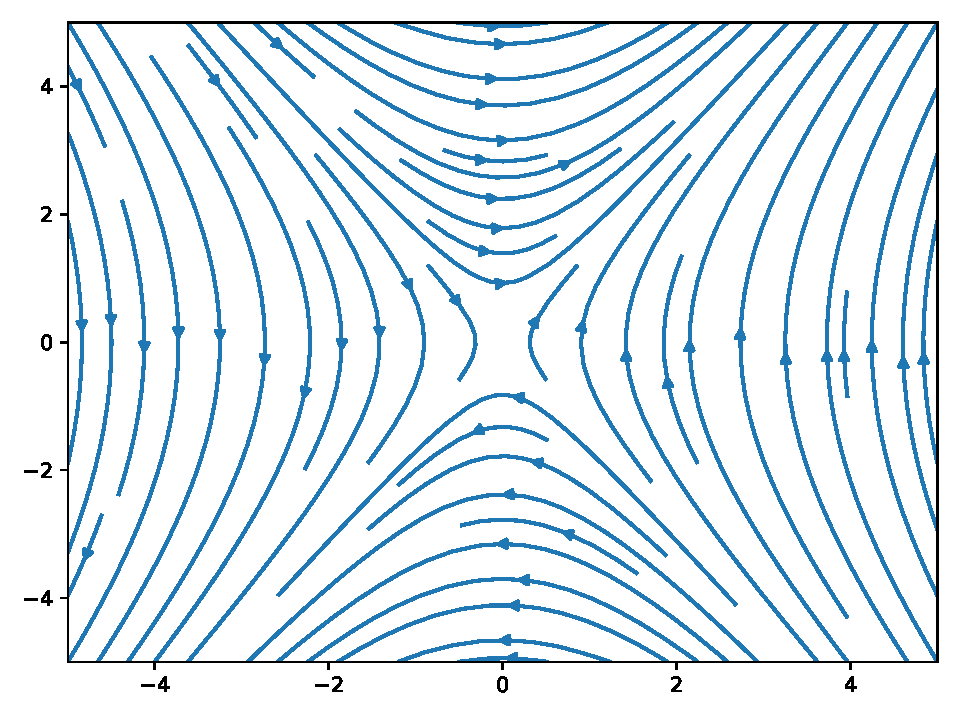
\includegraphics[width=.7\textwidth]{plots/ex5_fieldlines.pdf}
    \caption{Plot of the magnetic field lines ($\B = \left<y, \alpha^2x,
    0\right>$) using streamplot from python. We
    can see that that nullclines are at a different angle due to the parameter
    $\alpha$ ($> 1$), which according to the lorentz force will cause a net force acting
    on the fluid (i.e. magnetic pressure and tension are no longer aligned).}
\end{figure}
This phenomenon is very interesting and often referred to as Magnetic
Reconnection which is the complex phenomenon of how the nullclines of magnetic
fields are moved around by outside circumstances. 

\subsection{Magnetic Energy (Density)}
We can obtain an equation for the magnetic energy density similar to how a
kinetic energy equation is obtained for the velocity field.
\begin{gather*}
    E_M = \int_V\frac{|\B^2|}{2\mu_0}dV \\
    \frac{\B}{\mu_0} \cdot \left( \ppt{\B} = -\grad\times\E\right)\\
    \ppt{}\left(\frac{|\B|^2}{2\mu_0}\right) =
    -\frac{\B}{\mu_0}\cdot\grad\times\E\\
    \ppt{}\left(\frac{|\B|^2}{2\mu_0}\right) =
    -\frac{1}{\mu_0}\left(\grad\cdot(\E\times\B) +
    \E\cdot(\grad\times\B)\right)\\
    \ppt{M} =
    -\frac{1}{\mu_0}\int_S(\E\times\B)\cdot\nvec dS - \int_V
    \uvec\cdot(\jvec\times\B) - \frac{\jvec^2}{\sigma} dV
\end{gather*}
Here we can analyze each component of this magnetic energy density equation. We
have the ``Poynting vector`` $\E\times\B$ which represents the flux of magnetic
energy into the domain. We have the rate of magnetic energy loss by the
mechanical work against the lorentz force $\uvec\cdot(\jvec\times\B)$, and
finally ``Ohmic dissipation'' $\jvec^2/\sigma$. 


\subsection{Magnetohydrostatics}
We reintroduce the concept of balanced equations for hydrostatic balances, but
in the specific context for MHD. We look at the zero-velocity steady state flow
field. We must have some dominant balance in the navier stokes equation, 
\begin{gather*}
    0 = -\grad p + \rho \bs{g} + \jvec\times\B
\end{gather*}
This balance is denoted magnetohydrostatic balance and it relies on a very
important assumption that the timescales of interest for this problem are much
shorter than a diffusion timescale for the magnetic field. Note that the
velocity field doesn't necessarily have to be zero, but it must satisfy some
basic properies which make its relative magnitude negligable in the navier
stokes equation. 

Some common speeds used in physics scenarios are the following,
\begin{gather*}
    \left(\frac{\gamma p_0}{\rho_0}\right)^{1/2}, \quad \text{speed of sound}\\
    \left(\frac{B_0}{\mu_0\rho_0}\right)^{1/2}, \quad \text{Alfv\'en speed}\\
    \left(2g_0l_0\right)^{1/2}, \quad \text{gravity free fall speed}
\end{gather*}
where we must have $u$ is much less than these quantities in order to preserve
magentohydrostatic balance. Furhtermore there are several ways to obtain
hydrostatic balance from the magnetohydrostatic balance. Namely, we could have
$\B = 0$, $\jvec\times\B = $, or $\jvec = 0$ (in this case $\B$ can be written by
a potential function $\B = \grad A$). 

Some examples of force free fields are Beltrami fields, where $\grad\times\B =
\alpha(x) \B$ which is of course perpendicular to $\B$ at all points in space.
We find, 
\begin{gather*}
    \grad\cdot(\grad\times\B) = 0 = \div{\alpha\B} \\
    = \alpha(\div{\B}) + \B\cdot\grad\alpha \implies \B\cdot\grad\alpha = 0
\end{gather*}
let us assume for now that $\alpha$ is some constant. We have the following, 
\begin{gather*}
    \grad\times(\grad\times\B) = \alpha^2\B\\
    \grad(\grad\cdot\B) - \grad^2\B = \alpha^2\B\\
    \grad^2\B + \alpha^2\B = 0
\end{gather*}
which is a linear helmholtz equation for the magnetic field. Where as, solving
for a force free field by $\jvec\times\B = 0$ is much more difficult due to
nonlinearity. 

\section{Magnetohydrostatics: Continued}
\subsection{Review of Magnetohydrostatic balance}
We remember the equation for Magnetohydrostatic balance, whereby a steady state
inviscid flow is given by the balance between pressure, buoyancy/gravity, and
the lorentz force. Similarly, in the induction equation we only have magnetic
diffusion affecting the magnetic field. Thereby, the magnetic field will decay
and thus the magnetohydrostatic balance will erode and return to hydrostatic
balance. Note that in order for hydrostatic balance to be useful, we must
consider timescales much shorter than the magnetic diffusion timescale. 
\begin{gather*}
    0 = -\grad p + \rho\bs{g} + \jvec\times\B\\
    \ppt{\B} = \eta\grad^2\B
\end{gather*}

\subsection{Non-forcefree solutions}
Let us consider a simplified case to solve these equations whereby we have,
\begin{gather*}
    \B\cdot\left( 0 = -\grad p + \jvec\times\B\right), \quad \beta =
    \frac{p_{\text{gas}}}{p_{\text{mag}}}\\
    0 = \B\cdot\grad p\\
    \jvec\cdot\left( 0 = -\grad p + \jvec\times\B\right) \to 0 =
    \jvec\cdot\grad p
\end{gather*}
this tells us, as the original equation implies, that both $\B$ and $\jvec$ lie
within surfaces of constant pressure, and therefore $\jvec\times\B$ is parallel
to the gradients of pressure everywhere. Essentially this balance begs the
physical intuition of pressure balancing the lorentz force. 

\subsection{The Theta-Pinch}
\begin{gather*}
    \jvec = J\hat{\bs{\theta}}, \quad \B = b(r)\hat{\bs{r}}\\
    \jvec = \frac{1}{\mu_0}\grad\times\B =
    \frac{1}{\mu_0}\pp{b(r)}{r}\thetahat\\
    \jvec\times\B = \frac{1}{\mu_0}\left|\begin{array}{c c c}
                    \rhat & \thetahat & \zhat \\
                    0 & -\pp{b}{r} & 0\\
                    0 & 0 & b\end{array}\right|\\
                  = -\frac{b}{\mu_0}\frac{db}{dr}\rhat
\end{gather*}
With some algebra, we can show that $\ldots$.
Thus we obtain the conclusion that at some point,
\begin{gather*}
    \frac{b^2}{2\mu_0} = p_0 \implies p_{\text{gas}} = 0 
\end{gather*}

\subsection{Linear Pinch}

\begin{gather*}
    \B = b(r)\thetahat\\
    \jvec = \frac{1}{\mu_0r}\left|\begin{array}{c c c}
            \rhat & \thetahat & \zhat \\
            \pp{}{r} & \pp{}{\theta} & \ppz{}\\
            0 & rb(r) & 0\end{array}\right|\\
            = \frac{1}{\mu_0 r}\pp{rb}{r}\zhat\\
    \jvec\times\B = \frac{1}{\mu_0r}\left|\begin{array}{c c c}
            \rhat & \thetahat & \zhat \\
            0 & 0 & \pp{rb}{r}\\
            0 & b & 0\end{array}\right|\\
            = -\frac{b}{\mu_0r}\pp{rb}{r}\rhat
\end{gather*}

In order to solve this equation we first write

This solves the problem inside the radius of $a$ where there is current.
\begin{gather*}
    \jvec = J_0\zhat \\
    \pp{rb}{r} = J_0\mu_0r\\
    rb = \frac{J_0\mu_0}{2}r^2 + c_1\\
    b(r) = \frac{J_0\mu_0}{2}r + \frac{c_1}{r}\\
    b_i(r) = \frac{J_0\mu_0}{2}r, \quad r \le a
\end{gather*}
Outside of this current region we have a different solution and must solve for
continuity at the interface. 
\begin{gather*}
    \pp{rb}{r} = 0\\
    b_o(r) = \frac{c_1}{r} \to \frac{J_0\mu_0 a^2}{2r}, \quad r > a
\end{gather*}
We next want to understand how this solution affects the gas pressure in the
system. 
\begin{gather*}
    \frac{dp}{dr} = -\frac{b}{\mu_0r}\frac{d(rb)}{dr}\rhat\\
    \vdots\\
    p = \begin{cases}
        p_{\text{atmos}} & r > a\\
        -\frac{1}{4}J_0^2\mu_0(r^2-a^2)+p_{\text{atmos}} & r \le a\end{cases}
\end{gather*}

\subsection{Cylindrical Pinch}
The cylindrical pinch requires that the magnetic field has both an angular
component and a vertical component, i.e. 
\begin{gather*}
    \B = b_L\thetahat + b_T\zhat\\
    \jvec = J_T\thetahat + J_L\zhat\\
    -\pp{p}{r} - \pp{}{r}\left(\frac{b_L^2 + b_T^2}{2\mu_0}\right) -
    \frac{b_L^2}{\mu_0r} = 0
\end{gather*}
We can solve for the amount of twist in the system using the equations for the
fieldlines. 
\begin{gather*}
    \frac{d\theta}{dz} = \frac{b_L}{rb_T}\\
    \int d\theta = \frac{Lb_L}{rb_T}
\end{gather*}

\subsection{Reverse Field Pinch}
This idea stems from the Beltrami cylindrical geometry, 
\begin{gather*}
    \B = \left(0, B_{\theta}, B_z\right)\\
    \grad^2\B + \alpha\B = 0\\
    B_{\theta} = B_0J_0(\alpha r), \quad \text{this is a bessels function of
    order zero}\\
    B_{z} = B_0J_1(\alpha r), \quad \text{this is a bessels function of
    order one}
\end{gather*}


\section{Dynamics for MHD: Continued}

\subsection{Steady State MHD}
    Let us consider a simplified dynamical regime in which we encounter a steady
    state flow, i.e. $\ppt{\uvec} = 0$. We have that the governing equations
    reduce to the following:
\begin{gather*}
    (\uvec\cdot\grad)\uvec = -\frac{1}{\rho_0}\grad p + \jvec\times\B + \nu\grad^2\uvec\\
    \DDt{\B} = (\B\cdot\grad)\uvec + \eta\grad^2\B\\
    \grad\cdot\uvec = 0, \quad \div{\B} = 0
\end{gather*}
Next we consider a specific flow field $\uvec$ called the Hartmann flow given by
$\uvec = \left(u, 0, 0\right)$ and a specific magnetic field given by $\B = (0,
0, B_0)$. Let us investigate the dynamics that arise from this scenario.
At $t = 0$ we have that $\ppx{u} = 0$ and $\ppz{B_0} = 0$. Therefore, 
\begin{gather*}
    0 = -\frac{1}{\rho_0}\grad p + \frac{1}{\mu_0\rho_0}\left(\ppz{b} - \ppx{B_0}\right)\left(B_0\ex
    - b\ez\right)+ \nu\frac{\partial^2 u}{\partial z^2}\\
    u\ppx{b}\ex + u\ppx{B_0}\ez = B_0\ppz{u}\ex + \eta\grad^2B_0\ez  +
    \eta\grad^2b\ex\\
    \ppx{b} + \ppz{B_0} = 0,\quad  \ppx{u} = 0
\end{gather*}
This problem has boundary conditions $u(z+d) = 0$ and $u(z-d) = 0$ where d
is half of the height of the tube, and there is no boundary in the x-direction
(implicitly indicating it is an infinite tube). With these conditions, we cannot
presume any dependence on $x$ in the velocity field, nor the magnetic field
perturbations $b$. Thus we obtain the solution given by, 
\begin{gather*}
    u(z) = \left(\frac{p_0 + \sigma B_0E_0}{\sigma B_0^2}\right)\left(1 -
    \frac{\cosh(Mz/d)}{\cosh(M)}\right)\\
    \ddz{b} = \frac{E_0 - uB_0}{\eta} \\
    b(z) = \frac{E_0z}{\eta} - \left(\frac{p_0 + \sigma B_0E_0}{\eta\sigma
    B_0}\right)\left(z -
    \frac{d\sinh(Mz/d)}{M\cosh(M)}\right)
\end{gather*}
where $M$ is the Hartmann number given by $M = B_0/\sqrt{\mu\mu_0\eta}$ (measures
lorentz force against viscous diffusivity and $E_0$ is the $y$-component of
the given electric field) and $\mu$ is the permeability and $\mu_0$ is the
viscosity. 

\section{Dynamics for MHD: Continued}
\subsection{Steady State MHD and Hartmann flows}
    As a result of studying Hartmann flows, we obtain the Hartmann number
    which describes the relative weight of the lorentz force to the viscous
    diffusion of the flow. Most importantly, like any non-dimensional number,
    we have two limits which describe extreme regimes of dynamics. We have
    either $M \ll 1$ or $M\gg 1$. Let us investigate the solution to the
    Hartmann flow problem in either regime. 
\begin{align*}
    \frac{\cosh{Mz/d}}{\cosh{M}} &\sim \frac{\left(1 + \frac{(Mz/d)^2}{2} +
    \cdots\right)}{\left(1 + \frac{M^2}{2} + \cdots\right)}\\
    &\sim \left(1 + \frac{(Mz/d)^2}{2} +
    \cdots\right)\left(1 - \frac{M^2}{2} + \cdots\right)\\
    &\sim 1 - \frac{M^2}{2} + \frac{(Mz/d)^2}{2} + \cdots\\
    &\sim 1 - \frac{M^2}{2}\left(1 - \frac{z^2}{d^2}\right) + \cdots
\end{align*}
We can substitute this back into the solution for $u(z)$ we obtained in the last
lecture. We have, 
\begin{align*}
    u(z) &= \left(\frac{p_0 + \sigma B_0E_0}{\sigma
    B_0^2}\right)\left(\frac{M^2}{2}\left(1 - \frac{z^2}{d}\right)\right)\\
    &= \frac{1}{2\mu}\left(p_0 + \sigma B_0E_0\right) \left(d^2-z^2\right)
\end{align*}
This is the given solution in the limit of $M \ll 1$. We can redo this
computation in the limit where $M \gg 1$. In this scenario we have, 
\begin{align*}
    \cosh(x) &= \frac{e^x + e^{-x}}{2} \approx \frac{1}{2}e^{|x|}\\
    \frac{\cosh{Mz/d}}{\cosh{M}} &\sim \begin{cases} e^{|Mz/d| - |M|} &
    \left|\frac{Mz}{d}\right| \gg 1\\O(e^{-M}) &
    \left|\frac{Mz}{d}\right| < O(1)\end{cases}
\end{align*}
we notice that the $\cosh$ term is small everywhere except where $(1 - |z/d|)$
is also small, i.e. close to the boundary. Thus our solution reduces to a
constant flow field (with the constant given by the prefactor in front of the $1
- \cosh$ term), with a small boundary layer with a scale height given by $d$. We
can rescale our main variable, $z = d - \epsilon$, where $\epsilon$ is the
distance from the boundary such that $0 < \epsilon \ll 1$. We have, 
\begin{align*}
    \cosh(Mz/d) &= \cos\left(M(1 - \epsilon/d)\right) \sim e^{-M\epsilon/d}\\
    u(\epsilon) &\sim \left(\frac{p_0 + \sigma B_0E_0}{\sigma
    B_0^2}\right)\left(\frac{M\epsilon}{d} + \cdots\right)
\end{align*}
This solution gives a flow field which is asymptotically constant except within
the boundary layers which are given by a scale height $\frac{d}{M}$. This can be
seen in Figure \ref{fig:hartmann}. 
\begin{figure}
    \centering
    \includegraphics[width=\textwidth]{plots/bl_hartmann.pdf}
    \caption{Plot of the Steady State Hartmann flow with $M = 10$ $d = 1$ which
    shows the boundary layers created in the flow}
    \label{fig:hartmann}
\end{figure}

\subsection{Controlling flow and field with current}

Let us consider an electric field in a given three-dimensional domain $y \in
[-L, L]$. Let us consider, a simple Ohm's law given by $j = \sigma(\E + \uvec
\times \B)$ and a given electric field $\E = (0, E_0, 0)$, magnetic field $\B =
(0, 0, B_0)$, and  unidirectional flow
$\uvec = u(z)\ex$. Next we will perform an
average in the $z$ direction of the $y$ component of the current. 
\begin{gather*}
    I_y = \frac{1}{2d}\int_{-d}^{d} j_y dz = \sigma E_0 + \sigma
    B_0\int_{-d}^{d} u(z)dz\\
    = \sigma E_0 + \sigma
    B_0\overline{u}
\end{gather*}
This integral has cases. For example, given an open circuit we have that $I_y =
0$ whereby $\bar{u} = E_0/B_0$. This will act as a flow meter. Another example
is that of a short circuit, for example shorting the circuit by connecting the
two ends with another fire. We will have $E_0 = 0$ and therefore $j_y =
-u(z)B_0$. Let us consider the Lorentz force in the $x$-direction according to
this scenario. We have, 
\begin{gather*}
    \left(\jvec\times\B\right)_x = -j_zB_y + j_yB_z = -u(z)B_0^2
\end{gather*}
which will act as a negative definite term and resist the flow field. 

Another example could be introducing a small EMF (particularly $E_0 <
\bar{u}B_0$). Then we have, $j_y < 0$ and specifically, we have created an
electric generator, that is, the mechanical energy of the fluid drives a current
and this generates electrical energy. Note, that in this scenario the Lorentz
force would be negative as well. 

Finally, we could consider a large EMF (specifically larger than $\bar{u}B_0$).
This would create a positive current and thus a positive Lorentz force. 

\subsection{Waves}
In order to investigate waves in MHD, we must review waves in their most general
conceptualization. For example, the wave equation is classically defined as, 
\begin{gather*}
    \pptwo{\eta}{t} = c^2\pptwo{\eta}{x}
\end{gather*}
which is a hypervolid PDE and is governed by a parameter $c$ which is generally
thought of as the phase speed of the wave. The wave equation has some very
general solutions, for example D'Alembert's solution for the wave equation given
by $u(x,t) = f(x-ct) + f(x + ct)$ which is obtained by rewriting the wave
equation as the superposition of two transport equations ($\ppt{} \pm c\ppx{}$).
Most important about waves is their typical solutions. The periodicity of waves
often yields solutions of the form $\sin$ and $\cos$, i.e. fourier
eigenfunctions. This often simplifies the wave equation into an eigenvalue
problem which can be solved for multiple BC forms and problem setups.
Additionally, we can use Euler's identity to write general solutions as, 
\begin{gather*}
    u(x,t) = \sum_{k,\omega} A_{k,\omega}e^{i(kx - \omega t)}
\end{gather*}
D'Alemberts solution is non-dispersive (for $c$ constant). However, there are
many disperive waves, i.e. they might not have constant phase and group speeds.
If we return to the wave equation and use an ansatz to solve for the angular
velocity and wavenumber we obtain a dispersion relation, 
\begin{gather*}
    \ppt{\eta} + c\ppx{\eta} +\alpha\pp{^3\eta}{x^3} = 0
    -i\omega + c(ik) - \alpha ik^3 = 0 \implies \frac{w}{k} = c - k^2
\end{gather*}
This is the phase speed, and in constrast the group speed is given by
$\pp{\omega}{k}$. These are general wave properties and each of them apply to
the waves studied in other contexts. Specifically in MHD, there are several
restoring forces which can be used to generate waves. Alfv\'en waves are generated
by magnetic tension. Compressional Alfv\'en waves are generated by magnetic
pressure. Surface/internal gravity waves are generated by
gravity/stratification. Acoustic waves ar generated by pressure gradients.
Inertial waves are typically generated by the coriolis force. 

\section{Waves in MHD: Shear Alfv\'en Waves}

\subsection{Elastic Waves on a String}
Let us consider a string which has elasticity that is plucked. We can consider a
2D problem where the string only oscillates up and down (not forward and
backwards). The restoring force becomes the tension in the string rather than
gravity. Thus any displacements from equilibrium will be acted on by tension. We
can immagine the force acting on either ends of an infinitesimal length of
string $ds$. On either end we have $T_1$ and $\alpha_1$ and $T_2$ and $\alpha_2$
which  are the amplitide of tension and the angle with respect to the horizontal
that the tension acts in. In the scenario where there is no Left-Right motion we
have, 
\begin{gather*}
    T_2\cos(\alpha_2) = T_1\cos(\alpha_1)
\end{gather*}
and in the case where we have Up-Down motion (i.e. a standing wave), 
\begin{gather*}
    T_2\sin(\alpha_2) - T_1\sin(\alpha_1) = \frac{\rho \delta x}{T}\pptwo{y}{t}\\
    \tan(\alpha_2)-\tan(\alpha_1) = \frac{\rho \delta x}{T}\pptwo{y}{t}\\
    \frac{1}{\delta x}\left( \ppx{y}{x}|_{x+\delta x} - \ppx{y}{x}|_{x}\right) =
    \frac{\rho}{T}\pptwo{y}{t}\\
    \pptwo{y}{x} = \frac{\rho}{T}\pptwo{y}{t}
\end{gather*}
Thus we obtain a wave equation for a transverse wave. We could consider the case
where rather than a physical string, we consider the perturbation of magnetic
field lines, in which case the restoring force is magnetic tension. In this case
we replace the dummy variable $T$ with magnetic tension. 
\begin{gather*}
    \pptwo{y}{t} = \frac{B_0^2}{\rho\mu_0}\pptwo{y}{x}, \quad v_A =
    \sqrt{\frac{B_0^2}{\rho\mu_0}}
\end{gather*}
We can obtain this result with a formal analysis. Consider an incompressible,
undamped, IDEAL, fluid without the affects of gravity nor rotation. 
\begin{gather*}
    \rho_0\left(\DDt{\uvec}\right) = -\grad p + \jvec\times\B, \quad \div{\uvec}
    = 0\\
    \DDt{\B} = (\B\cdot\grad)\uvec, \quad \div{\B} = 0
\end{gather*}
Let us assume a basic state for the flow, which we take to be magnetohydrostatic
balance. Thus we have, 
\begin{gather*}
    0 = -\grad p + \jvec\times\B
\end{gather*}
and consider the perturbations to the flow, i.e. $\uvec = \overline{\uvec} + \uvec'$,
and specifically $\overline{\uvec} = 0$.
\begin{gather*}
    \rho_0\left(\DDt{\uvec'}\right) = -\grad p' +
    \overline{\jvec}\times\B' + \jvec'\times\overline{\B}+\jvec'\times\B', \quad \div{\uvec'}
    = 0\\
    \ppt{}(\overline{\B} + \B') = \grad\times(\uvec'\times\overline{\B}) +
    \grad\times\uvec'\times\B', \quad \div{\overline{\B} + \B'} = 0
\end{gather*}
After linearizing with the fact that $|\B'| \ll |\overline{\B}|$ and taking
$\overline{\B}$ to be steady, we have
\begin{gather*}
    \rho_0\left(\ppt{\uvec'} \right) = -\grad p' +
    \overline{\jvec}\times\B' + \jvec'\times\overline{\B}, \quad \div{\uvec'}
    = 0\\
    \ppt{\B'} = \grad\times(\uvec'\times\overline{\B}), \quad \div{\B'} = 0
\end{gather*}
We can simplify the problem more if we simply take $\overline{\B}$ to be a constant
field. 
\begin{gather*}
    \rho_0\left(\ppt{\uvec'} \right) = -\grad p' +
    \jvec'\times\overline{\B}, \quad \div{\uvec'}
    = 0\\
    \ppt{\B'} = \grad\times(\uvec'\times\overline{\B}), \quad \div{\B'} = 0
\end{gather*}
Then using a vector identity to simplify the triple vector product, 
\begin{gather*}
    \rho_0\left(\ppt{\uvec'} \right) = -\grad \left(p' +
    \frac{1}{\mu_0}\B'\cdot\overline{\B}\right) + \frac{1}{\mu_0}(\overline{\B}\cdot\grad)\B', \quad \div{\uvec'}
    = 0\\
    \ppt{\B'} = (\overline{\B}\cdot\grad)\uvec', \quad \div{\B'} = 0
\end{gather*}
thus we obtain lineared, momentum and induction equations which contain a
typical magnetic pressure and tension term (products of $\overline{B}$ and $\B'$) and
in the induction equation a typical linearized evolution equation. In order to
get rid of the pressure terms, we will take the curl of the two obtained
equations. We have, 
\begin{gather*}
    \rho_0\left(\ppt{\bs{\omega}'} \right) = (\overline{\B}\cdot\grad)\jvec' \\
    \ppt{\jvec'} = \mu_0(\overline{\B}\cdot\grad)\bs{\omega}'
\end{gather*}
Now can can combine these equations by taking additional derivatives and then
use substitution to obtain. 
\begin{gather*}
    \pptwo{\bs{\omega}'}{t} =
    \frac{1}{\mu_0\rho_0}(\overline{\B}\cdot\grad)^2\bs{\omega}'\\
    \pptwo{\jvec'}{t} = \frac{1}{\mu_0\rho_0}(\overline{\B}\cdot\grad)^2\jvec'
\end{gather*}
Further investigation into the RHS reveals that for a uniform vertical magnetic
field we have, $(\overline{\B}\cdot\grad)^2 = B_0^2\pptwo{}{z}$. Thus we have
found a wave equation with a well defined wavespeed for transverse waves of the
perturbations to magnetic field lines. 

\subsection{Searching for Wavelike Solutions from the linearized equations}
Let us investigate this problem from the perspective of an ansatz considering
the equations have constant coefficients. 
\begin{gather*}
    q' = \tilde{q}e^{i\bs{k}\cdot\x - \omega t}
\end{gather*}
Let us plug this into our linearized equations, 
\begin{gather*}
    -\rho_0\omega\tilde{\uvec} = -\bs{k}\left(\tilde{p} +
    \frac{1}{\mu_0}\tilde{\B}\cdot\overline{\B}\right) +
    \frac{1}{\mu_0}(\overline{\B}\cdot\bs{k})\tilde{\B}, \quad
    \bs{k}\cdot\tilde{\uvec}
    = 0\\
    -\omega\tilde{\B} = (\overline{\B}\cdot\bs{k})\tilde{\uvec}, \quad
    \bs{k}\cdot\tilde{\B} = 0
\end{gather*}
Similar to the last setup, we will take the curl of these two equations
$\grad\times = \bs{k}\times$, 
\begin{gather*}
    -\rho_0\omega\bs{k}\times\tilde{\uvec} =
    \frac{1}{\mu_0}(\overline{\B}\cdot\bs{k})\bs{k}\times\tilde{\B}\\
    -\omega\bs{k}\times\tilde{\B} = (\overline{\B}\cdot\bs{k})\tilde{\uvec}
\end{gather*}
Now using substitutions we can show, 
\begin{gather*}
    -\rho_0\omega\bs{k}\times\frac{-\omega\tilde{\B}}{\overline{\B}\cdot\bs{k}} =
    \frac{1}{\mu_0}(\overline{\B}\cdot\bs{k})\bs{k}\times\tilde{\B}\\
    \frac{\rho_0\omega^2}{\overline{\B}\cdot\bs{k}}\bs{k}\times\tilde{\B} =
    \frac{1}{\mu_0}(\overline{\B}\cdot\bs{k})\bs{k}\times\tilde{\B}\\
    \omega^2 = \frac{1}{\rho_0\mu_0}(\overline{\B}\cdot\bs{k})^2 =
    \frac{1}{\rho_0\mu_0}|\overline{\B}|^2|\bs{k}|^2\cos^2(\theta)
\end{gather*}
This is a dispersion relation for these MHD waves. We notice a few things. First
and foremost, the wavespeed is fastest when the wavevector is parallel to
$\overline{\B}$. Secondly, there is no propagation when the wavevector is
perpendicular to $\overline{\B}$. These statements are originate from the
geometry of the dot product. We can also consider the phase and group speed for
these waves,
\begin{gather*}
    c = \frac{\omega}{\bs{k}} = v_A^2|\bs{k}|\cos^2(\theta)\\
    c_g = \pp{\omega}{\bs{k}} = 2 v_A^2 \frac{\bs{k}^2}{|\bs{k}|}\cos^2(\theta)
\end{gather*}
An interesting way to visualize this dispersion relation is a polar diagram of
the dispersion relation. 


\section{Waves for MHD: Continued}
\subsection{Compressible Alfv\'en Waves}
We are going to search for Compressible Alfv\'en waves and look for waves in the
same manner, assume a small perturbation to the field and then linearize the
equations about that perturbation. Then solve for a dispersion relation or
something or other. Now though, since density isn't constant we need an equation
of state. We will consider
\begin{gather*}
    p = p(\rho), \quad p = \rho^{\gamma}, \quad \gamma = \frac{c_p}{c_v} \\
    \delta p = \gamma\rho^{\gamma -1} \delta \rho\\
    p' = \gamma\frac{\overline{p}}{\overline{\rho}}\rho'
\end{gather*}
We continue from our lineariized equations as before but now with a more complex
density and pressure. 
\begin{gather*}
    \overline{\rho}\left(\ppt{\uvec'} \right) = -\grad \left(p' +
    \frac{1}{\mu_0}\B'\cdot\overline{\B}\right) + \frac{1}{\mu_0}(\overline{\B}\cdot\grad)\B'\\
    \ppt{\B'} = (\overline{\B}\cdot\grad)\uvec', \quad \div{\B'} = 0\\
    \ppt{\rho'} + \grad\cdot(\overline{\rho}\uvec') = 0, \quad p' = c_s^2\rho'
\end{gather*}
We will proceed that $\overline{\B}$ is uniform (and its derivative is zero
everywhere). We proceed with a wave-like ansatz and investigate the linearized
equations. 
\begin{gather*}
    -\overline{\rho}\omega\tilde{\uvec} = -\bs{k}\left(\tilde{p} +
    \frac{1}{\mu_0}\tilde{\B}\cdot\overline{\B}\right) +
    \frac{1}{\mu_0}(\overline{\B}\cdot\bs{k})\tilde{\B}\\
    -\omega\tilde{\B} = (\overline{\B}\cdot\bs{k})\tilde{\uvec}, \quad
    \bs{k}\cdot\tilde{\B} = 0\\
    -\omega\tilde{\rho} + \overline{\rho}\bs{k}\cdot\tilde{\uvec} = 0\\
    \tilde{p} = c_s^2\tilde{\rho}
\end{gather*}
Let us confirm that without the magnetic components that a solution exists.
\begin{gather*}
    -\overline{\rho}\omega\tilde{\uvec} = -\bs{k}c_s^2\tilde{\rho}\\
    -\omega\tilde{\rho} + \overline{\rho}\bs{k}\cdot\tilde{\uvec} = 0
\end{gather*}
We can show that we obtain a dispersion relation in this scenario whereby we
have, 
\begin{gather*}
    -\omega^2\tilde{\rho} + \overline{\rho}\left(\bs{k} \cdot
    \frac{+\bs{k}c_s^2\tilde{\rho}}{\omega\overline{\rho}}\right) = 0\\
    -\omega^2\tilde{\rho} + \bs{k}^2c_s^2\tilde{\rho}= 0\\
    \omega^2 =  \bs{k}^2c_s^2\\
    \left(\frac{\omega}{\bs{k}}\right)^2 = c_s^2
\end{gather*}
Now we can move on to the more complicated case with the inclusion of magnetic
effects. We go back to the complete set of linearized equations. 
\begin{gather*}
    -\overline{\rho}\omega\tilde{\uvec} = -\bs{k}\left(\tilde{p} +
    \frac{1}{\mu_0}\tilde{\B}\cdot\overline{\B}\right) +
    \frac{1}{\mu_0}(\overline{\B}\cdot\bs{k})\tilde{\B}\\
    -\omega\tilde{\B} = (\overline{\B}\cdot\bs{k})\tilde{\uvec}, \quad
    \bs{k}\cdot\tilde{\B} = 0\\
    -\omega\tilde{\rho} + \overline{\rho}\bs{k}\cdot\tilde{\uvec} = 0, \quad \tilde{p} = c_s^2\tilde{\rho} 
\end{gather*}
From these equations we obtain the result given by, 
\begin{gather*}
    \left(\omega^2 - (c_s^2 + v_A^2)\bs{k}^2\right)\tilde{\uvec}\cdot\bs{k} = -
    \frac{(\overline{\B}\cdot\bs{k})(\overline{\B}\cdot\tilde{\uvec})}{\mu_0\rho_0}\\
    \left(\omega^2 \right) = \\
    \omega^2\left(\tilde{\uvec}\cdot\overline{\B}\right) =
    (\tilde{\uvec}\cdot\bs{k})c_s^2(\bs{k}\cdot\overline{\B})\\
    \left(\frac{\omega^2}{\bs{k}^2}\right)^2 -
    \left(c_s^2+v_A^2\right)\frac{\omega^2}{\bs{k}^2} + c_s^2v_A^2\cos^2\theta =
    0
\end{gather*}
This dispersion relation reveals two cases (depending on the roots of the
quadratic given). In the $+$ sign regime, we have fast magnetoacoustic waves
wherein gas pressure and magnetic pressure act together and contribute
productively towards the wavespeed, whereas in the $-$ sign regime they
contribute destructively and produce slow magnetoacoustic waves. 
\begin{gather*}
    \frac{\omega^2}{\bs{k}^2} = \frac{1}{2}\left[c_s^2 + v_A^2 \pm (v_A^2 - c_s^2)\right]
\end{gather*}

\subsubsection{The Cold Limit}
The cold limit can be described by taking the limit as the sound speed goes to
zero (i.e. the air is so cold that acoustic waves cannot be propagated).  We
have, 
\begin{gather*}
    \frac{\omega^2}{\bs{k}^2} = \frac{1}{2}\left(v_A^2\pm v_A^2\right)
\end{gather*}
and in this case we either have a wavespeed given by the Alfv\'en speed or no wave
speed at all. Notice however that unlike Shear Alfv\'en waves this disperasion
relation is independent of $\cos(\theta)$ and is therefore isotropic. This is
techinically denoted a ``Compressional Alfv\'en Wave'' thought it might be more
aptly described as an ``Magnetoacoustic Wave in the limit of $c_s \to 0$''. More
general examples of Magnetoacoustic waves is given by the Eric Priest book
``Solar MHD'' and Chandrasehkar's book ``Hydrodynamic and Magnetohydrodynamic
stability''. 


\section{Instabilities in MHD}

\subsection{Linear Instabilities}
The first consideration when it comes to instabilities in fluid mechanics is
typically the notion of a linear instability caused by a perturbation. We could
imagine a parabolic energy slope. If the slope is an parabola which opens up the
extreme value is a minumum and perturbations away from that minimum will
oscillate around that minimum by restoring force. That is, the ampltitude of the
pertubation oscillates but does not grow in time. If the parabola downs down, a
perturbation away from that maximum will continue to fall down the parabola,
i.e. tending towards an energetic minimum, and the amplitude of oscillation
grows exponentially in time, hence instability. 

There is another case called non-linear instability whereby by a finite
amplitude pertubation we might find a region of different stability which is
inaccessible by infinitesimal perturbations. These landscapes tend to originate
from nonlinearity in the governing equations. 

\subsection{Common Hydrodynamic Instabilities}
The Rayleigh-Taylor instability is a common instability whereby two fliud bodies
separated by an interface whereby the compositional or thermal gradient is
oriented as to be energetically unstable. In this regime, we find that some sort
of convection must occur in order to rearrange the gradient to be in a stable
configuration. As an example, let us consider a wavelike perturbation to the
interface between two fluids. In the case where the higher density fluid is on
the bottom, the interface perturbation relaxes back to equilibrium. In the case
where the higher density fluid is on the top, the perturbation to the interface
leads to convective plumes and an interchange and perhaps destruction of the
interface completely occurs. 

When a magnetic field is present and the fluid is highly conducting, we find
that the presence of a unidirectional magnetic field might stabilize the
Rayleigh-Taylor instability, whereby magnetic pressure and tension will suppress
the perturbation of the fluid due to the stretching and movement of the field
lines. There are two different modes of the instability which depend on the
alignment of the magnetic field. Let us say that the field is pointing in the
x-direction. We have then that the instability modes with $k_x = 0$ are called
interchange modes, whereas the modes with $k_x \ne  0$ are called undular modes. We
think of the undular modes being acted on by magnetic tension primarily and the
interchange modes being acted upon by the magnetic pressure primarily. By
performing a linear stability analysis we find the following dispersion
relation, 
\begin{gather*}
    \omega^2 = -g\bs{k}\left(\frac{\rho_{top} - \rho_{bot}}{\rho_{top} +
    \rho_{bot}}\right) + \frac{2B_0^2k_x^2}{\mu_0(\rho_{top}+\rho_{bot})}
\end{gather*}
Note that this dispersion relation may or may not yield complex values for the
angular frequency $\omega$ depending on the relative weight of the convective
instability compared the stabilizing effect of the magnetic field as illustrated
by the dispersion relation. 

Another popular instability is the Kelvin-Helmholtz instability, typically the result of a shear flow wherein the
interface between the velocity profiles induces small eddies which grow in time
as a result of a linear instability. 

\subsection{Magnetic Buoyancy}
The Parker 1955 paper was a paer that investigated the notion of magnetic
buoyancy whereby flux tubes containing internal properties isolated and
distinct from the
external properties. What Parker posited was that ther much be some magnetic
pressure which equilibriated the flux tube so that the total pressure is
the same as outside the flux tube. Parker found that the adjustment must
happen by the mechanism of a magnetoacoustic wave which is often the fastest
propagating sound/acoustic wave in the presence of a magnetic field. 

We can show that there must be a formal instability here and let us investigate
that. Let us take some quantities which vary with the height in the system, i.e.
$\rho = \rho(z)$, $\B = \B(z)$. Let us take the density to increase as the
height decreases, and the same for the magnetic field intensity. Let us take
that at some level in the domain we have the quantities $\rho_0, p_0, T_0, B_0$.
We now consider a blob which is lifted from that level without being able to
equilibrate. We have the properties of the blob are now, 
\begin{gather*}
    \rho_0 \to \rho_0 + \delta \rho\\ p_0\to p_0 + \delta p\\ T_0\to T_0 +
    \delta T\\ B_0\to B_0 + \delta B
\end{gather*}
Inside the blob, we do have to conserve mass. In order to do so we notice an
adjustment to the volume of the blob. 
\begin{gather*}
    \rho_0V_0 = (\rho_0+\delta\rho)(V_0+\delta V)\\
    (\rho_0+\delta\rho)\delta V = -\delta\rho V_0
\end{gather*}
There is also an adjustment to the flux and because flux must be conserved
through the tube, 
\begin{gather*}
    \rho_0V_0 = (\rho_0+\delta\rho)(V_0+\delta V)\\
    (\rho_0+\delta\rho)\delta V = -\delta\rho V_0
\end{gather*}
As a consequence we must have, 
\begin{gather*}
    \frac{d\rho}{\rho_0} = \frac{dB}{B_0}\\
    \frac{\delta p}{p_0} = \gamma \frac{\delta \rho}{\rho_0}\\
    (p_0+dp) + \frac{(B_0 + d B)^2}{2\mu_0} = (p+\delta p_0) + \frac{(B_0 + \delta
    B_0)^2}{2\mu+0}\\
    dp + \frac{B_0dB}{\mu_0} = \delta p_0 + \frac{B_0\delta B_0}{\mu_0}\\
    \delta\rho = \frac{\rho_0}{\gamma p_0}\delta p\\
    = \frac{\rho_0}{\gamma p_0}\left(dp + \frac{B_0dB}{\mu_0} - \delta p_0 +
    \frac{B_0\delta B_0}{\mu_0}\right)\\
    = \frac{\rho_0}{\gamma p_0}\left(dp + \frac{B_0dB}{\mu_0} - \delta p_0 +
    \frac{B_0^2\delta \rho_0}{\mu_0\rho_0}\right)\\
    \delta\rho\left(1 + \frac{B_0^2}{\mu_0\gamma p_0}\right) =
    \frac{\rho_0}{\gamma p_0}\left(dp + \frac{B_0dB}{\mu_0}\right)\\
    \delta\rho = \frac{\frac{\rho_0}{\gamma p_0}\left(dp +
    \frac{B_0dB}{\mu_0}\right)}{\left(1 + \frac{B_0^2}{\mu_0\gamma
    p_0}\right)}
\end{gather*}
Now that we have solved for $\delta\rho$ we must now satisfy the following
equality:
\begin{gather*}
    \delta \rho < d\rho\\
    \frac{\rho_0\left(dp +
    \frac{B_0dB}{\mu_0}\right)}{\left(\gamma p_0 + \frac{B_0^2}{\mu_0}\right)} < d\rho
\end{gather*}
This equation must be satisfied and it is perhaps more intuitive to divide by
$dz$ in which case all of the terms becomes vertical gradients of the background
profiles. After some simplifications we can obtain, 
\begin{gather*}
    \frac{d\rho}{dz} > \frac{-\rho_0 g}{\gamma \frac{p_0}{\rho_0} +
    \frac{B_0^2}{\rho_0\mu_0}} = \frac{-\rho_0 g}{c_s^2+v_A^2}
\end{gather*}
Alternatively we can consider the following inequality which is equivalent,
\begin{gather*}
    \left(c_s^2 + v_A^2 - 1\right) \frac{d\rho_0}{dz} >
    \frac{B_0}{\mu_0}\dd{B_0}{z}\\
    -v_A^2\left[\ddz{}\left(\ln(B_0)\right) -
    \ddz{}\left(\ln(\rho_0)\right)\right] > \ddz{}\left(\ln(p_0)\right) -
    \gamma\ddz{}\left(\ln(\rho_0)\right)\\
    -v_A^2\ddz{}\left(\ln\left(\frac{B_0}{\rho_0}\right)\right)>
    \ddz{}\left(\ln\left(\frac{p_0}{\rho^{\gamma}}\right)\right)
\end{gather*}


\begin{gather*}
\end{gather*}
\end{document}
